\documentclass[11pt]{article}
\usepackage{geometry} % see geometry.pdf on how to lay out the page. There's lots.
\usepackage{hyperref}
\usepackage{graphicx}
\usepackage{gensymb}
\usepackage[affil-it]{authblk}
\usepackage[toc,page]{appendix}
\usepackage{pifont}
\usepackage{amsmath}
%% \usepackage{draftwatermark}

%% \SetWatermarkText{DRAFT}
%% \SetWatermarkScale{6}
%% \SetWatermarkLightness{0.95}

% \geometry{letter} % or letter or a5paper or ... etc
% \geometry{landscape} % rotated page geometry

% See the ``Article customise'' template for come common customisations

\title{Gluss = Slug + Truss}
\author{Robert L. Read
  \thanks{read.robert@gmail.com}
}
\affil{Founder, Public Invention, an educational non-profit.}


\date{\today}

%%% BEGIN DOCUMENT
\begin{document}

\maketitle

%% \tableofcontents

\begin{abstract}
  An innovative approach to modular robotics that combines manipulation and locomotion is described.
  Extending the TETROBOT\cite{sanderson1996modular,lee2002dynamic,lee1999dynamics} concept of a variable-geometry
  space frame or truss composed only of joints and linear actuators with a new 3D-printable emodiment of a
  spherical joint\cite{song2003spherical}
  produces a completely modular mechanically strong tentacle-like machine capable of independent locomotion.
  We call this truss that can ooze like a slug a \emph{gluss}.
  The \emph{turret joint} is shown to theoretically support a maximum ratio of maximum actuator length to
  minimum actuator length of  $\varphi \equiv \frac{1 + \sqrt{5}}{2} \approx 1.618...$.
  The simplest glussbot capable of crawling and turning, the 3TetGlussBot, is constructed of
  inexpensive open-source modules comprising an Arduino Mega, a custom PCB, servo controller chips, and a Bluetooth module.
  A 3-module robot, the 5TetGlussBot, that uses spherical magnetic joints is described which oozes at ~27 cm/min (11 in/min).
\end{abstract}

\section{Introduction}

The best introduction to this paper is to watch the 2:10 minute video of the
walking robot, or \emph{glussbot}, which this paper describes:\\
\\
\indent \href{https://www.youtube.com/watch?v=zl0AEfxyVMw}{https://www.youtube.com/watch?v=zl0AEfxyVMw}.\\

\begin{figure}[!ht]
  \centering
%%    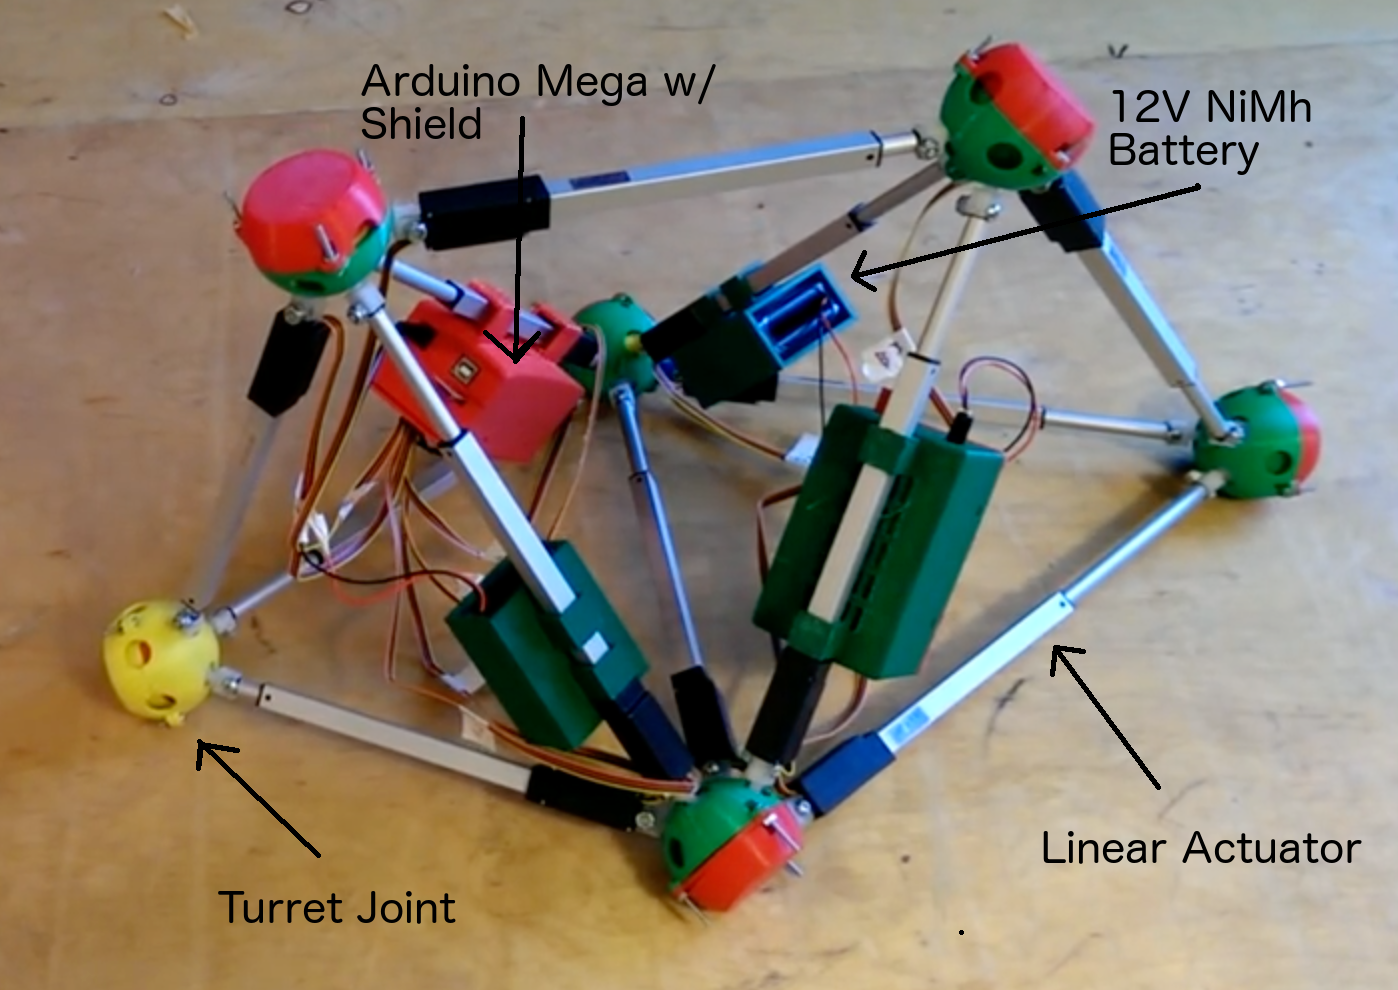
\includegraphics[width=0.8\textwidth]{figures/3TetGlussBotPhotoAnnotated.png}
    \caption[3TetGlussBot Components]{3TetGlussBot Components}
      \label{annotated}
\end{figure}


Between 14 and 21 years ago, Arthur C. Sanderson and his colleagues published a series of
papers\cite{sanderson1996modular,lee2002dynamic,lee1999dynamics} on modular robots.
The ``TETROBOT'' was a variable-geometry truss, in which motion was accomplished by the change
in length of linear actuators, connected in a modular geometry based on the tetrahedron and octahedron.  Such a system
requires a special joint which allows the actuators to remain aimed at the center of joints while supporting
a certain amount of rotation about this center.  The TETROBOT used a joint called the CMS joint.

This paper builds upon that work by introducing the concept of \emph{gluss}. It explains how to build it,
introduces 3D-printable embodiments of
a recently invented spherical joint\cite{song2003spherical}, 
and gives some results related to the underlying geometry and math, as well as providing
references to all of the open-source materials needed to duplicate and expand on this work. This is an
open-source embodiment of the TETROBOT with physically smaller actuators which is more accessible to the
hobbyist or researcher with a limited budget.  The development of 3D printers, Bluetooth, microprocessors
such as the Arduino, and inexpensive commercial actuators has made this possible.

\subsection{Motivation}

Imagine a strong, light, metamorphic material that can exert or resist force.
You can command it to form any shape, limited by its flexibility.
Using that power, you can, with some thought, get it to crawl across very rough terrain.
You can command it to form into a bridge or to lift and move heavy objects,
or to perform all the functions of a crane, a forklift, a backhoe and/or bulldozer.
It is a truss that crawls like a slug---a \emph{gluss}.
If you need more of it, you buy it by the kilo and when it arrives you order it
to crawl to your existing gluss. You easily join it there, creating a
larger, stronger, combined mass.

The advantages of snakebots have been widely recognized \cite{liljebäck2012snake}. In general, these have been constructed
with angular joints. In this paper we propose a different, truss-like approach to providing similar
mobility that uses only linear actuators and spherical joints that support no angular forces. This
potentially combines the advantages of forceful machines with snake-like mobility.

Other geometries, such as moving planes, are possible with the same material.

Other videos at the YouTube channel, Public Invention, reachable from the above link,
further motivate the \emph{gluss} concept.


\subsection{Concept: Gluss = Slug + Truss}

Imagine a metamorphic or polymorphic machine that forcefully assumes a variety of shapes. It moves like a mollusc or amoeba,
oozing into position as commanded. It is technically a ``machine'' because it can exert force reliably, but
it may be thought of as a material, because unlike most robots its components are not differentiated.

Although someday an actual chemical substance may do this, today it can be constructed from commercial components
and 3D-printable parts. This paper introduces the \emph{gluss} approach to building metamorphic dynamic robots
and static machines.\footnote{ ``Gluss'' is a portmanteau of ``Slug'' and ``Truss'' because we are attempting to
build a truss, or space frame, that is capable of moving like a slug or octopus.
The word \textit{gluss}
should be used as a substantive noun in English, much like the word \textit{clay} is used.
The use of \textit{glusses}, the plural
of \textit{gluss}, should be rare and refer to different kinds of metamorphic material, such as the expression
``four clays'' suggests four distinct types of clay without specifying how many kilograms of each one means.}

Massively scalable robots have often been proposed. Our particular approach is to use linear actuators,
which are rod-like machines that can make themselves shorter or longer. These are tied together using
a relatively new joint \cite{song2003spherical} which allows, for example, as many as 12, but more realistically 4 or 6,
members to be joined together sturdily at a single point.
A 3-D printed embodiment presented here, called the \emph{turret joint}, allows the
change of angle required for the gluss to ooze about. Some gluss consists of some actuators joined together
with some turret joints and whatever batteries and control microelectronics are needed. In the first
crawling robot discussed here, the \emph{3TetGlussBot}, there are two controllers and two batteries
in addition to the 12 actuators and the 6 multi-member turret joints, but 3TetGlussBot is only
a small amount of gluss compared to what we hope to build. Additionally, we present \emph{5TetGlussBot}, an obvious extension of the
3Tet geometry implemented with magnetic joints.

\begin{figure}[!ht]
  \centering
%%    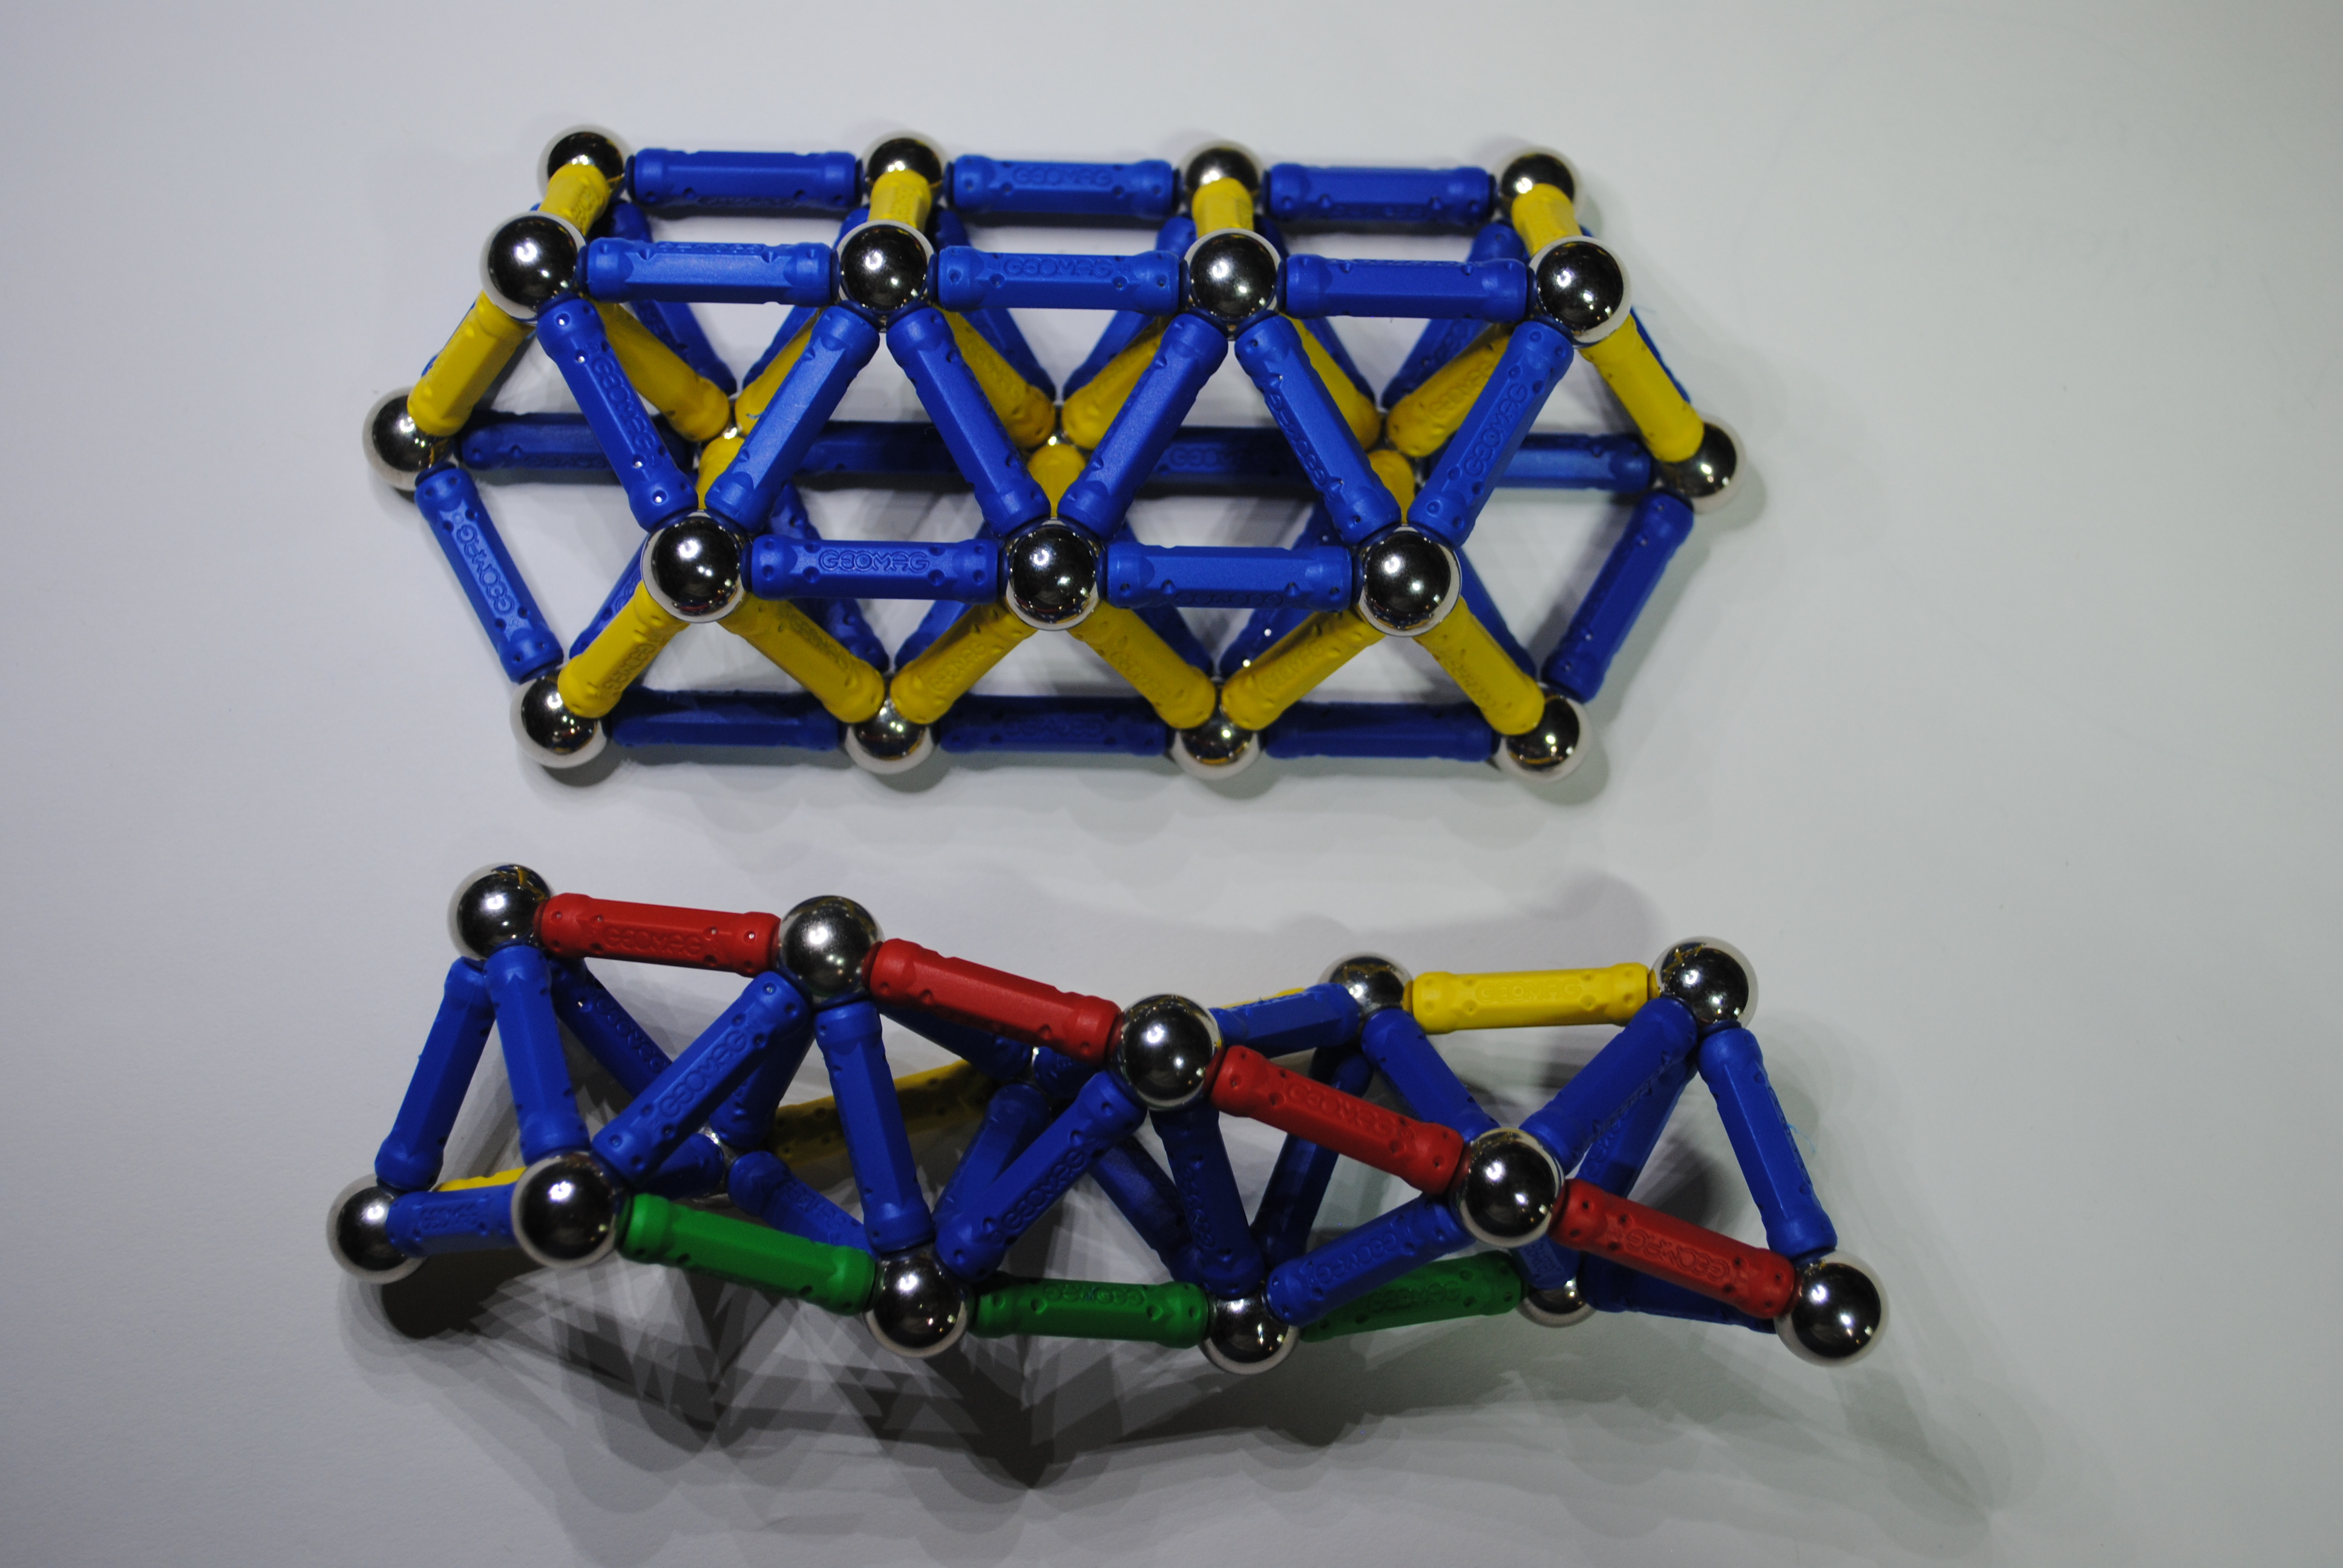
\includegraphics[width=1.0\textwidth]{figures/TwoGeometries.jpg}
    \caption[The Octet Truss (above) and Tetrahelix (below)]{The Octet Truss (above) and Tetrahelix (below)}
      \label{twogeometries}
\end{figure}


Although unlimited geometries are possible, two geometries (See Figure \ref{twogeometries}) 
have the advantage of being regular, thus allowing us to
seamlessly connect any number of actuators into any amount of gluss with some hope of effective software control.

\section{The \textit{Turret Joint}}

\subsection{The Need}

The way to make something large, light, and strong is to make it inherently rigid by building it
out of triangles. In a single plane, this is called a \emph{truss} \cite{ambrose1993building}, and more generally is called
a \emph{space frame}.  Space frames made completely from triangles tend to be rigid even if the
joints that connect members allow motion, such as a pin joint or a ball-and-socket joint. This
is an advantage because strain (that is, a slight change in the angular geometry of the frame) cannot cause
the joint to fail, as it can with a welded joint.

But we seek a space frame that can change its shape dramatically. Imagine a radio tower in which
each girder has been replaced with an actuator that can get longer or shorter. Such a tower could
bend its top down to the ground, or even
tie itself into a knot. To accomplish this, the joints must support significant although not
limitless range of angular motion. 

The spherical joint invented by Song, Kwon and Kim \cite{song2003spherical} is such a joint,
the essence of which is rendered in their patent drawing, Figure \ref{SongKwonKimImage}.
We name this joint the \emph{Turret Joint}.

\begin{figure}[!ht]
  \centering
%%    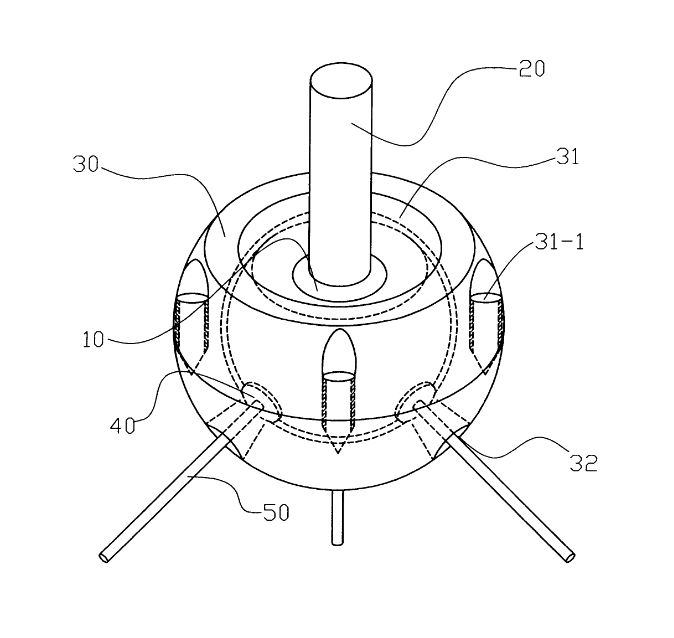
\includegraphics[width=0.5\textwidth]{figures/SongKwonKimImage.png}
    \caption[Song, Kwon, Kim, patent image.]{Song, Kwon, Kim, patent image.}
      \label{SongKwonKimImage}
\end{figure}

When properly configured to support regular nets of actuators,
it allows the gluss to be a moving space frame. It happens that the specific actuators we use
are geared such that when no power is applied, they strongly resist outside forces that would change their length,
essentially become rigid members.
The resulting gluss
can move into position and then be powered off to be a temporarily static space frame.

One could also use this joint with members which are not actuators. For example, we first
constructed the joint with carbon fiber rods. In essence it is then becomes a construction kit with continuously
variable member lengths liberated from using a finite set of angles.

\subsection{Geometry}

\begin{figure}[!ht]
  \centering
%%  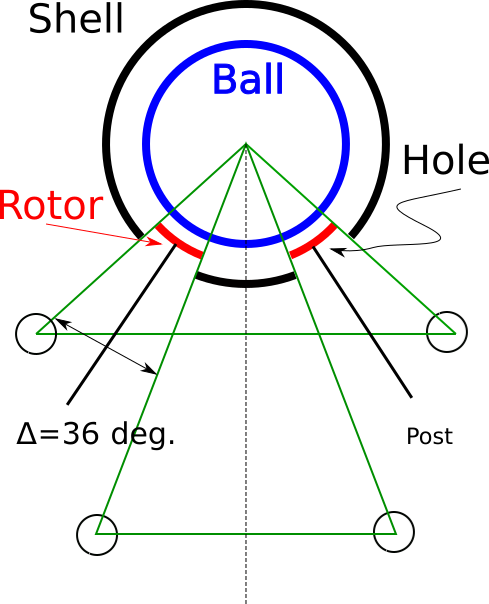
\includegraphics[width=0.5\textwidth]{figures/SimplifiedConstraintDrawing.png}
    \caption[Turret Joint Planar Geometry]{Turret Joint Planar Geometry}
      \label{simplified-constraint-drawing}
\end{figure}

How versatile can we make the turret joint?

In particular, since we are attempting to build gluss which is regular in its use of actuators, we may ask:
What is the maximum range of motion in our
actuators which we can usefully employ in our gluss?
To work independent of scale, we use the symbol $Q$ to denote the ratio of the actuator at its
longest to its length at its shortest.
The particular Actuonix actuators we use have a $Q$ of 1.5. But is that the maximum $Q$ that we could utilize? Or is
it already too high?

One way to approach this problem is to consider a single triangle formed by joints and actuators.
The joint must support the most acute triangle
that can be formed with the three actuators and the most obtuse triangle that can be formed with the actuators.

In fact it is a surprising result that we prove in Appendix A that the maximum $Q$ which can be utilized
by an ideal turret joint happens to be
the famous golden ratio, $\varphi \equiv \frac{1 + \sqrt{5}}{2} \approx 1.618...$, and the maximum deviation for any one member coming
into the joint is $36\degree$.
Thus in Figure \ref{simplified-constraint-drawing} the triangles drawn are in fact a Golden Triangle and a Golden Gnomon.
This is interesting but has little to
do with a real-world joint, which will support less variation because the ``post'' must have a
certain thickness and the ``rotor'' must have a lip
slightly larger than the hole in order to remain locked in place.
Furthermore, the joint adds a certain necessary thickness, the minimum length
 from joint-center to joint-center will be somewhat greater than from actuator tip to actuator tip.

 However, the theoretic result is a valuable guideline and makes a $Q$ for a physical actuator of 1.5 seem quite appropriate.

 \subsection{Embodiment}

 Although the joint could be machined or formed in some other way,
 3D Printers have made the construction of the Turret Joint far easier.
 We have designed a complete set of components needed to 3D print the joint and the rotors to attach to
 the linear actuators. These models are created with OpenSCAD, a functional parametric modeling program.

 Our experience has been that the common plastics PLA and ABS are adequate for the Turret Joint,
 but have found that nylon, which is far tougher and less prone to cracking, is superior for the
 rotors which bolt directly to the actuators.

 \begin{figure}[!ht]
  \centering
%%    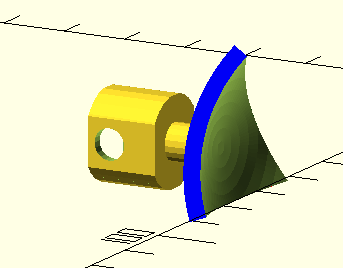
\includegraphics[width=0.5\textwidth]{figures/RotorModel.png}
    \caption[Triangular Rotor Model]{Triangular Rotor Model.}
      \label{rotormodel}
\end{figure}

 We have innovated the design of the rotor slightly by using a triangular section of a sphere as the
 rotor rather than a circular section, as shown in Figure \ref{rotormodel}.
 Assuming that each actuator is free to rotate about its axis as well as revolve about the
 center of the ball joint, this shape does not limit motion even in the most pinched
 configurations. The triangular rotor provides greater extent of contact,
 which presumably makes the joint motion
 smoother and less likely to bind.
 

 Figure \ref{parts} shows most of the parts. The nylon trinagular rotor is white and rests upon
 the red ball. The green part is a Tetrahelix lock, and the yellow parts are the locks for the Octet Truss
 geometry.

\begin{figure}[!ht]
  \centering
%%    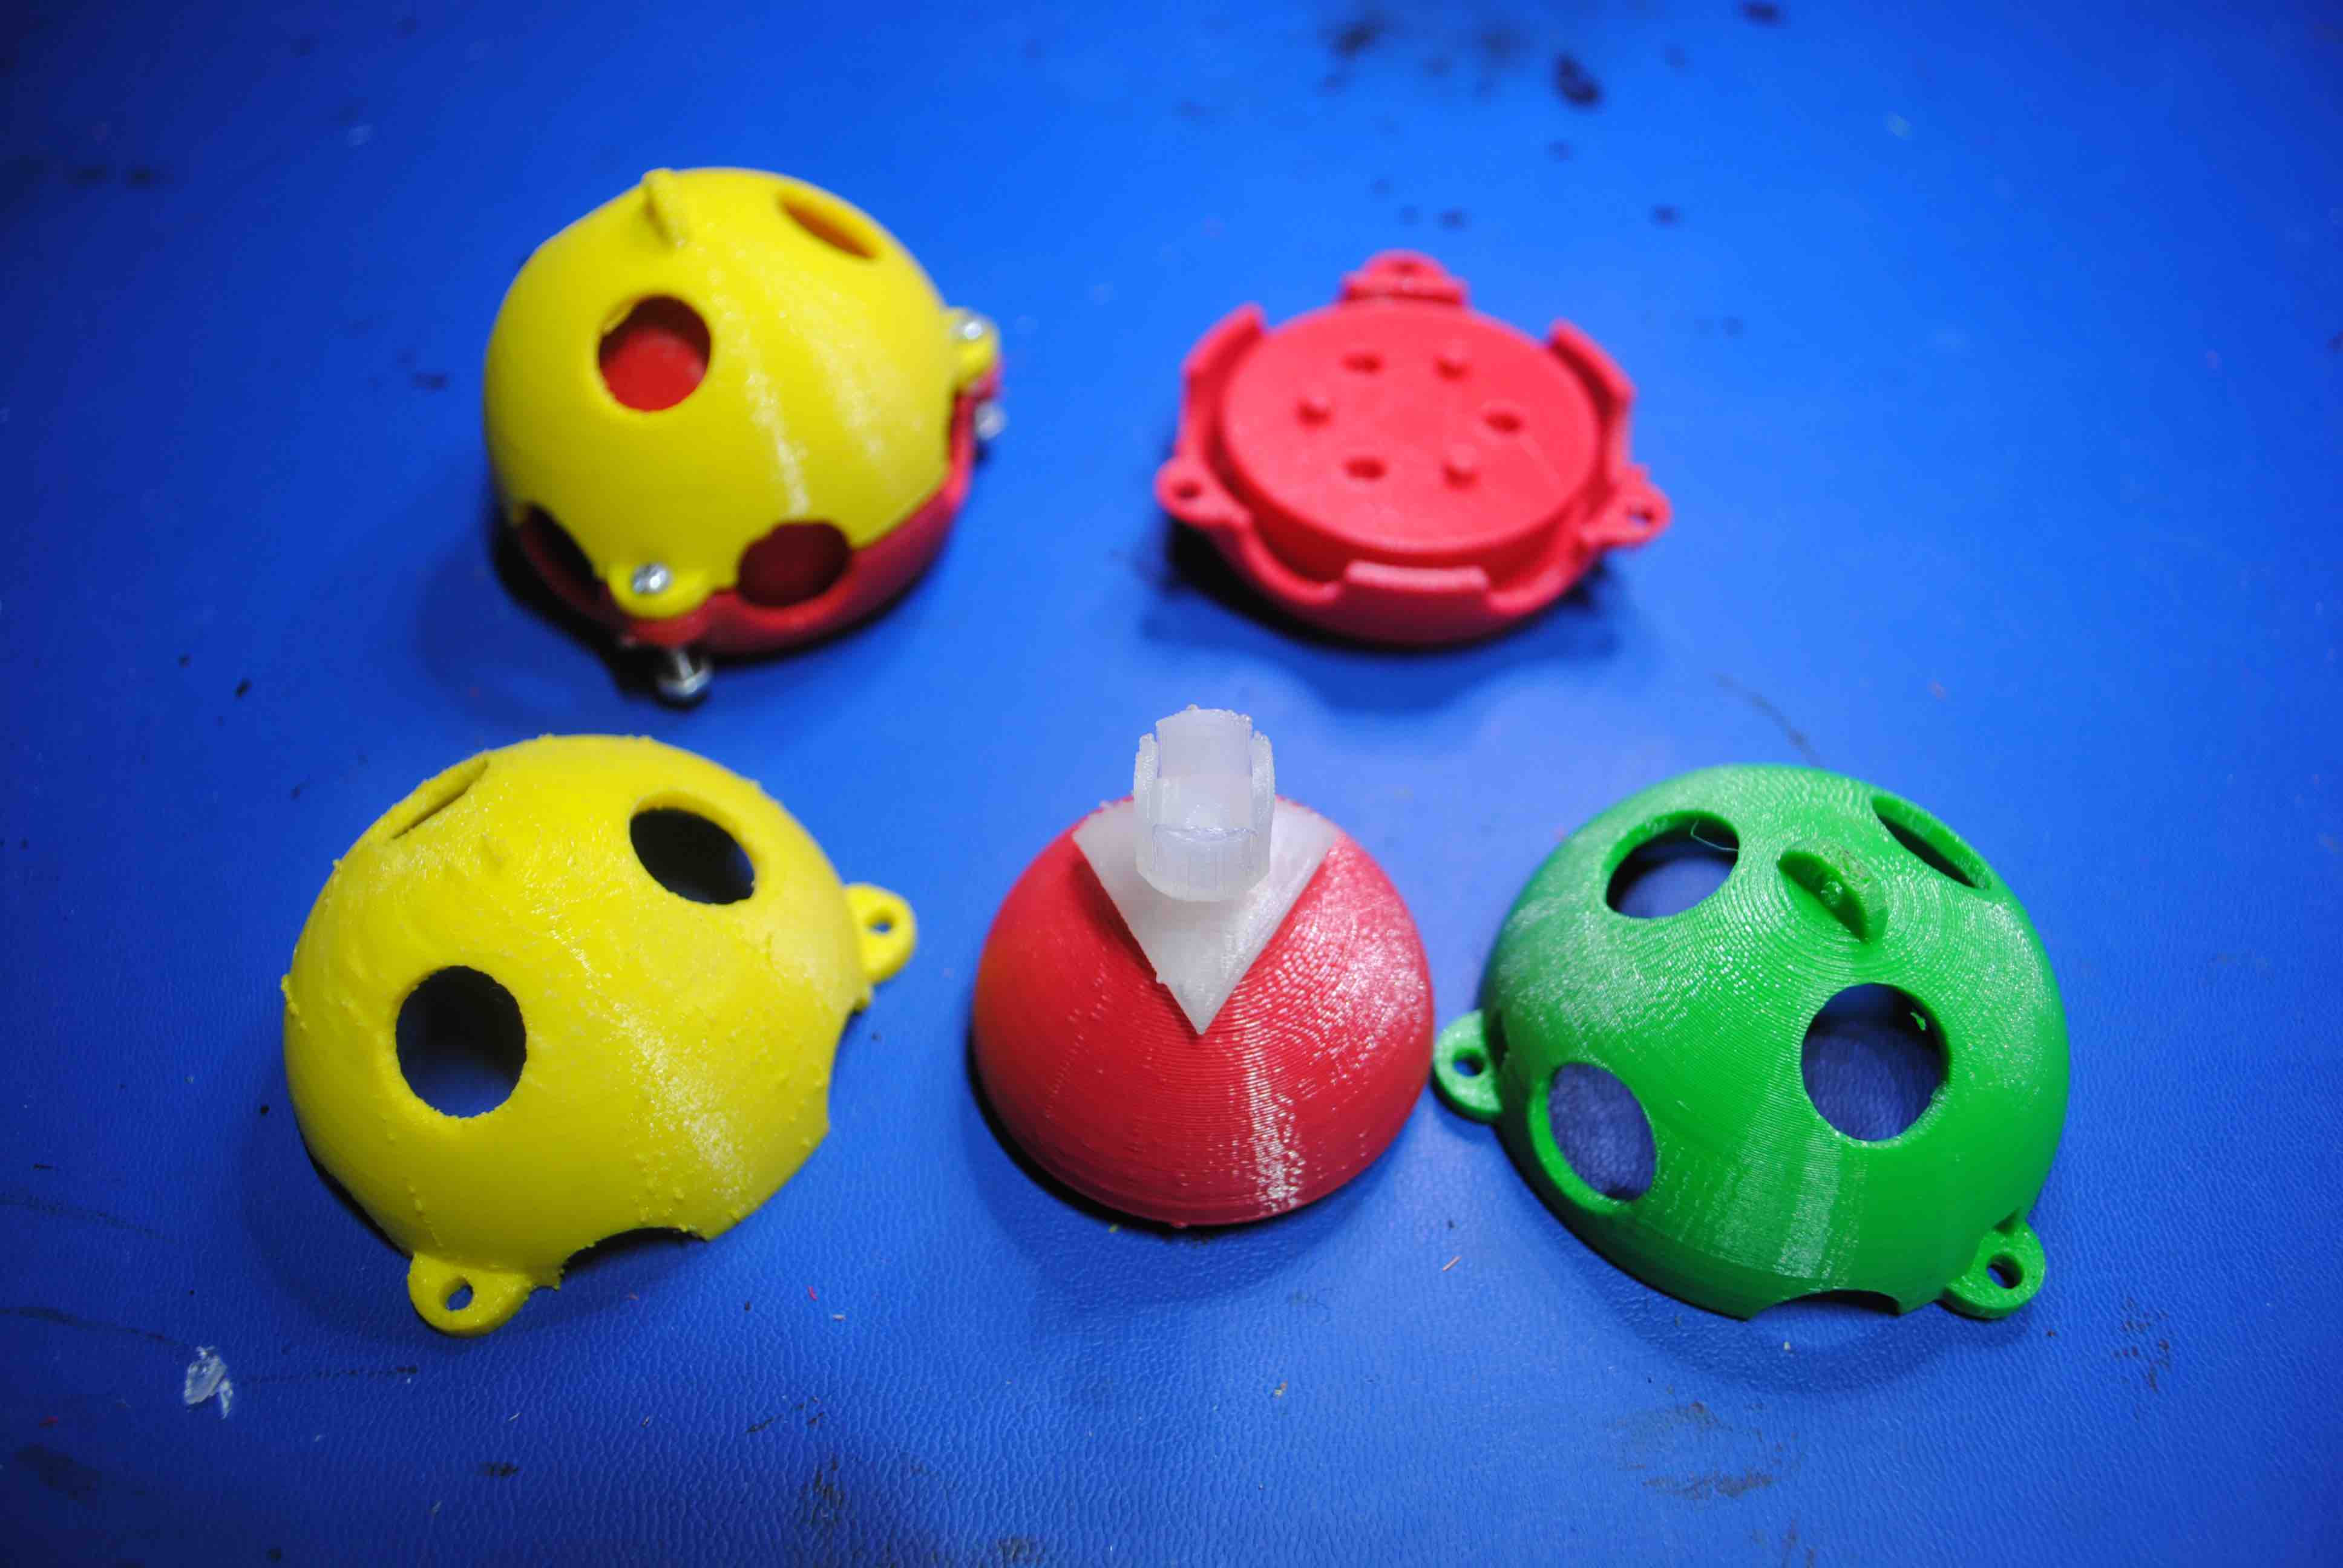
\includegraphics[width=0.7\textwidth]{figures/Parts.jpg}
    \caption[3D Printed Parts]{3D Printed Parts}
      \label{parts}
\end{figure}

In Section \ref{linearactuators}, one of our actuators and also a carbon rod with 3D-printed tubular mounts
is shown in Figure \ref{rodAndActuator}.
The carbon rod and mounts can be used as a construction system to build a static structure.
By cutting the rods to any length, you can build a static version of any geometry that the actuators
are capable of achieving.

\subsection{Specific Geometries}

Although the possible ways to configure actuators and joints is limitless, the simplest thing is to
use regular, repeatable geometries. The two most obvious are the Boerdijk--Coxeter helix
(more easily called the \textit{tetrahelix})
\url{https://en.wikipedia.org/wiki/Boerdijk%E2%80%93Coxeter_helix}
  and the \emph{Octet Truss}
  \cite{richard1961synergetic}.
  It is instructive to compare Figure \ref{octet-truss-patent} with the photo of the same object
  made with the GeoMag toy shown in Figure \ref{twogeometries}.
    
Roughly speaking, the Tetrahelix is a good way to make a long shaft or tentacle, and the octet truss
is a good way to make a planar shape. The purpose of a tentacle is to curl, and the we have no word for
a plane that roll itself up into a cylinder or cone or form a barrel vault. Buckminster Fuller discusses
both the tetrahelix and octet-truss \cite{fuller1982synergetics} in terms of static structures and geometries.

\begin{figure}[!ht]
  \centering
%%    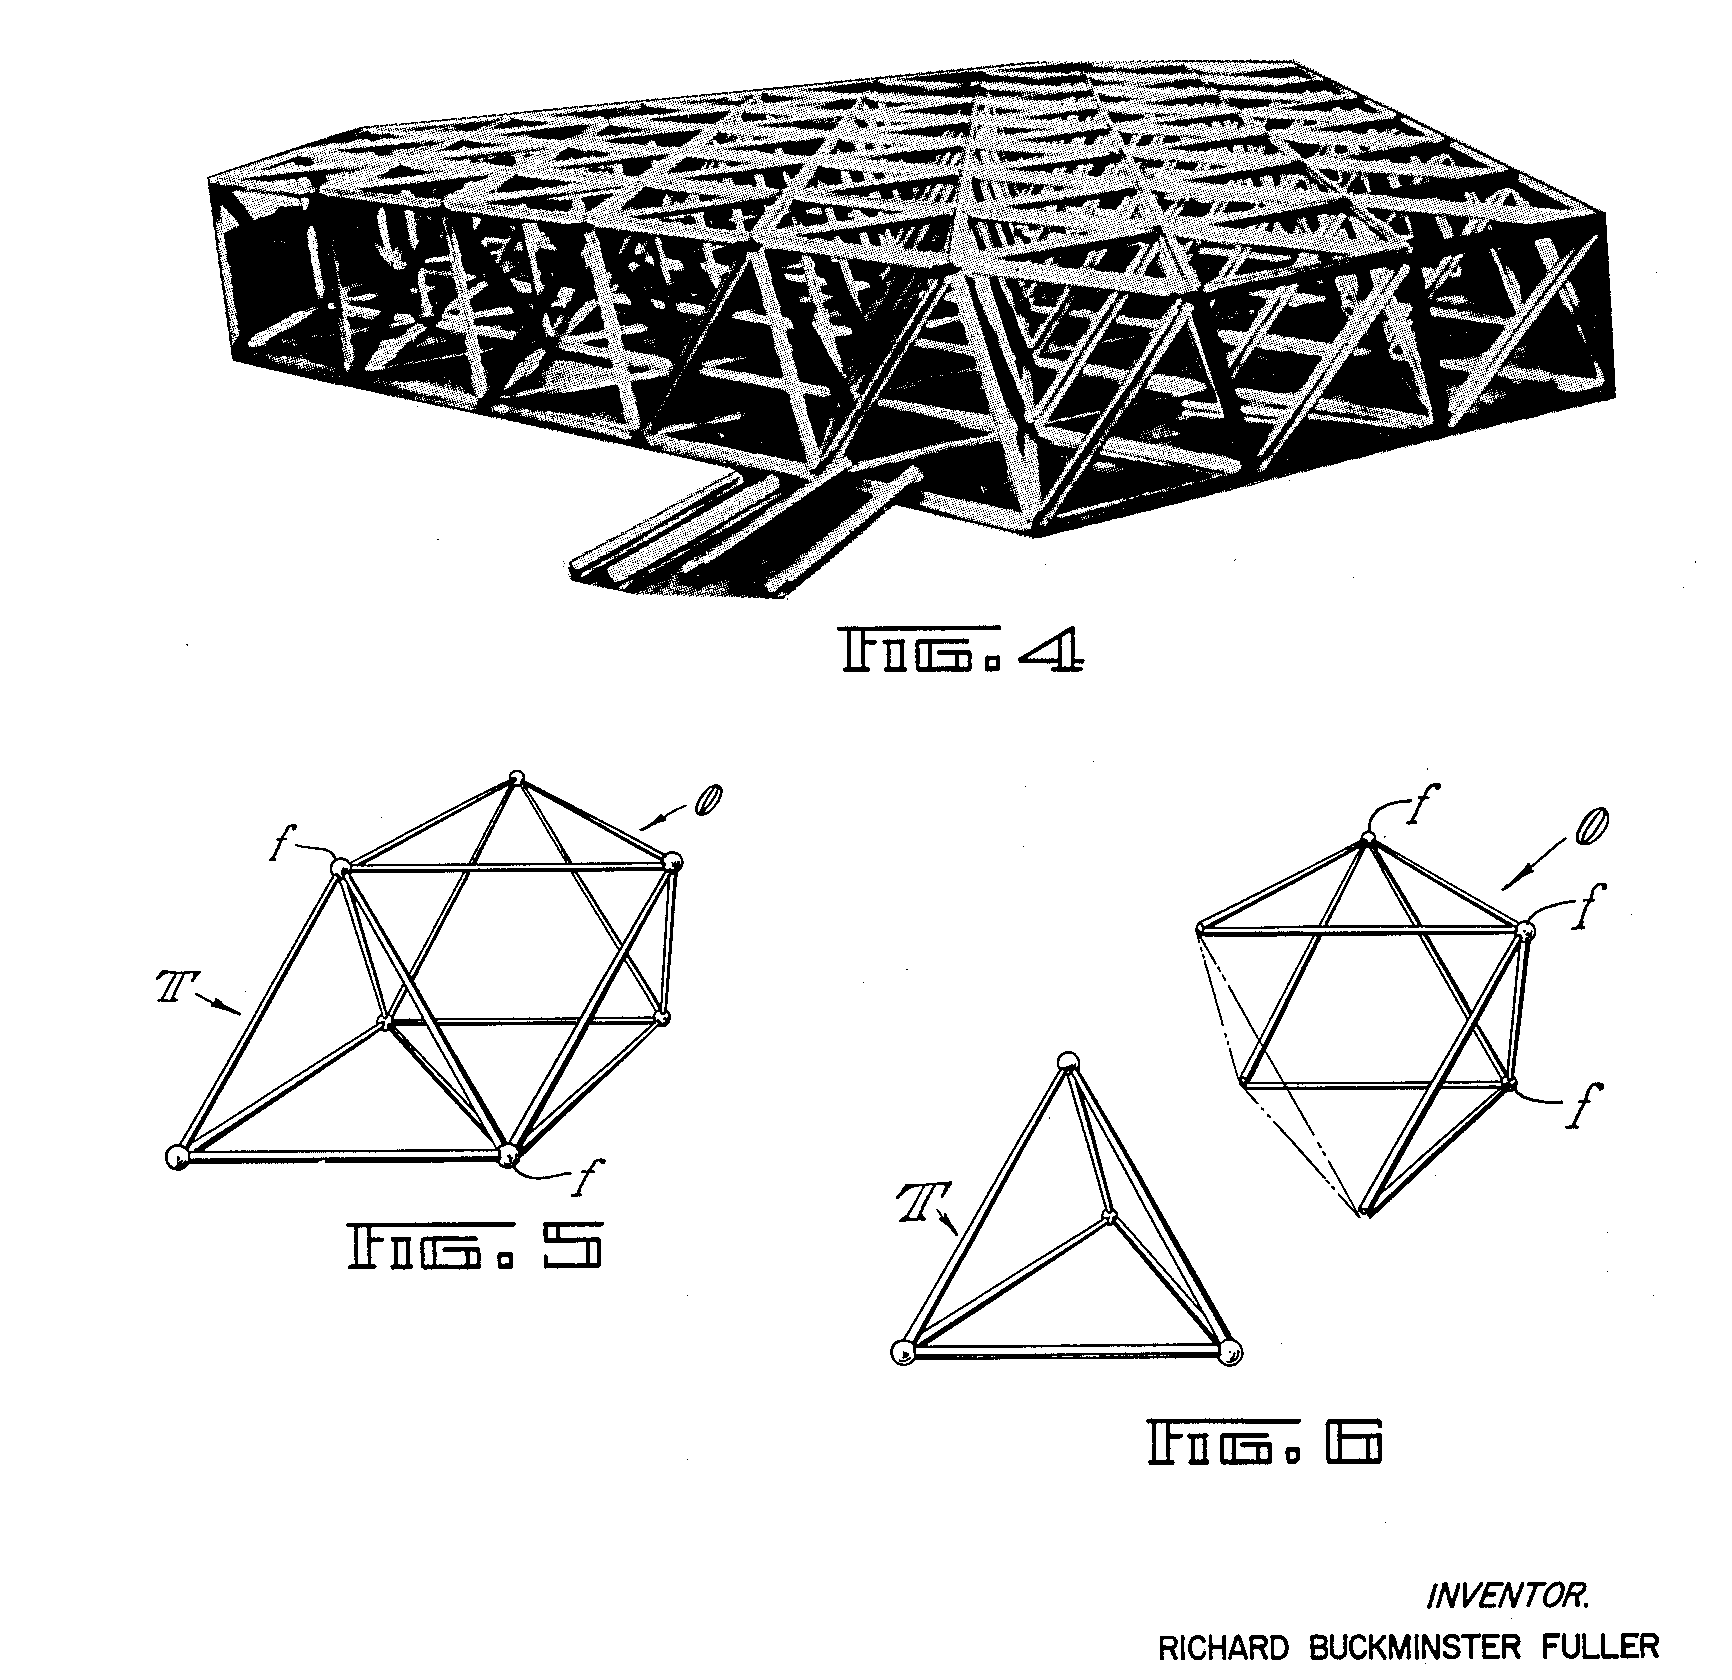
\includegraphics[width=0.5\textwidth]{figures/OctetTrussSelection.png}
    \caption[The Octet Truss]{The Octet Truss, selected from Buckminster Fuller's patent.}
      \label{octet-truss-patent}
\end{figure}

The Octet Truss reflects the geometry called the \emph{cuboctahedron}.

Because the Turret Joint does not support infinite revolution of all members, the joint, or the ``lock'' or ``stator'' in particular,
must be adjusted to the regular geometry that one is implementing.  The Figure \ref{lockcomparison} indicates this difference.
The image is from TurrentJoint.scad:\\
\href{https://github.com/PubInv/turret-joint/blob/master/Models/TurretJoint.scad}{https://github.com/PubInv/turret-joint/blob/master/Models/TurretJoint.scad}, an
open-source file that can be used to 3D print all of the turret joint components.
It shows a lock part for the Tetrahelix geometry
on the left, and the more expansive Octet Truss geometry on the right. Observe that some of the holes are half in this part,
and have in the ``cap'' parts not shown here.

\begin{figure}[!ht]
  \centering
%%    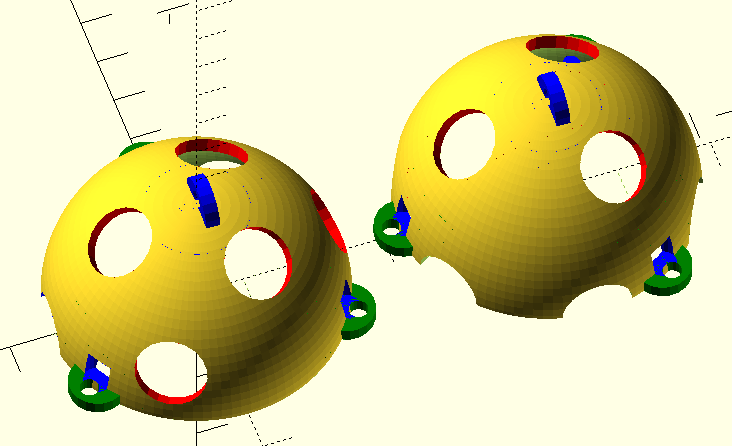
\includegraphics[width=0.5\textwidth]{figures/TetrahelixLockVsOctetTrussLock.png}
    \caption[Lock Comparison]{Lock Comparison}
      \label{lockcomparison}
\end{figure}


We have additionally experimented with magnetic joints similar to those use in the Geomag\textsuperscript{TM} toy.
These joints use 1/2'' diameter by 1'' long neodymium magnets restrained within small cages such that the circular face
may contact a 2'' diameter hollow steel ball.  This provides a pull force greater than the 50 Newton force applied by our linear
actuators. The \emph{5TetGlussBot} (see Figure \ref{5TetGlussBot}) using these
joints was demoed at the Wichita Mini Maker Faire July 30-31, 2016.

Although this joint functions well and easily achieves the intention of making the robot quick to assemble and
disassemble for travel,
it is easily broken by side forces.
Since climbing over obstacles and stairs will necessarily involve side forces on the actuators,
we intend to move away from the magnetic joints.

Furthermore, it would be very expensive to scale upward (and similarly becomes less expensive when
scaling downward.) We believe the magnetic joint could be a good engineering solution for glussbots smaller than the current
general scale of 50 Newton, 400mm-average-length actuators.


\section{Linear Actuators}
\label{linearactuators}

\begin{figure}[!ht]
  \centering
%%    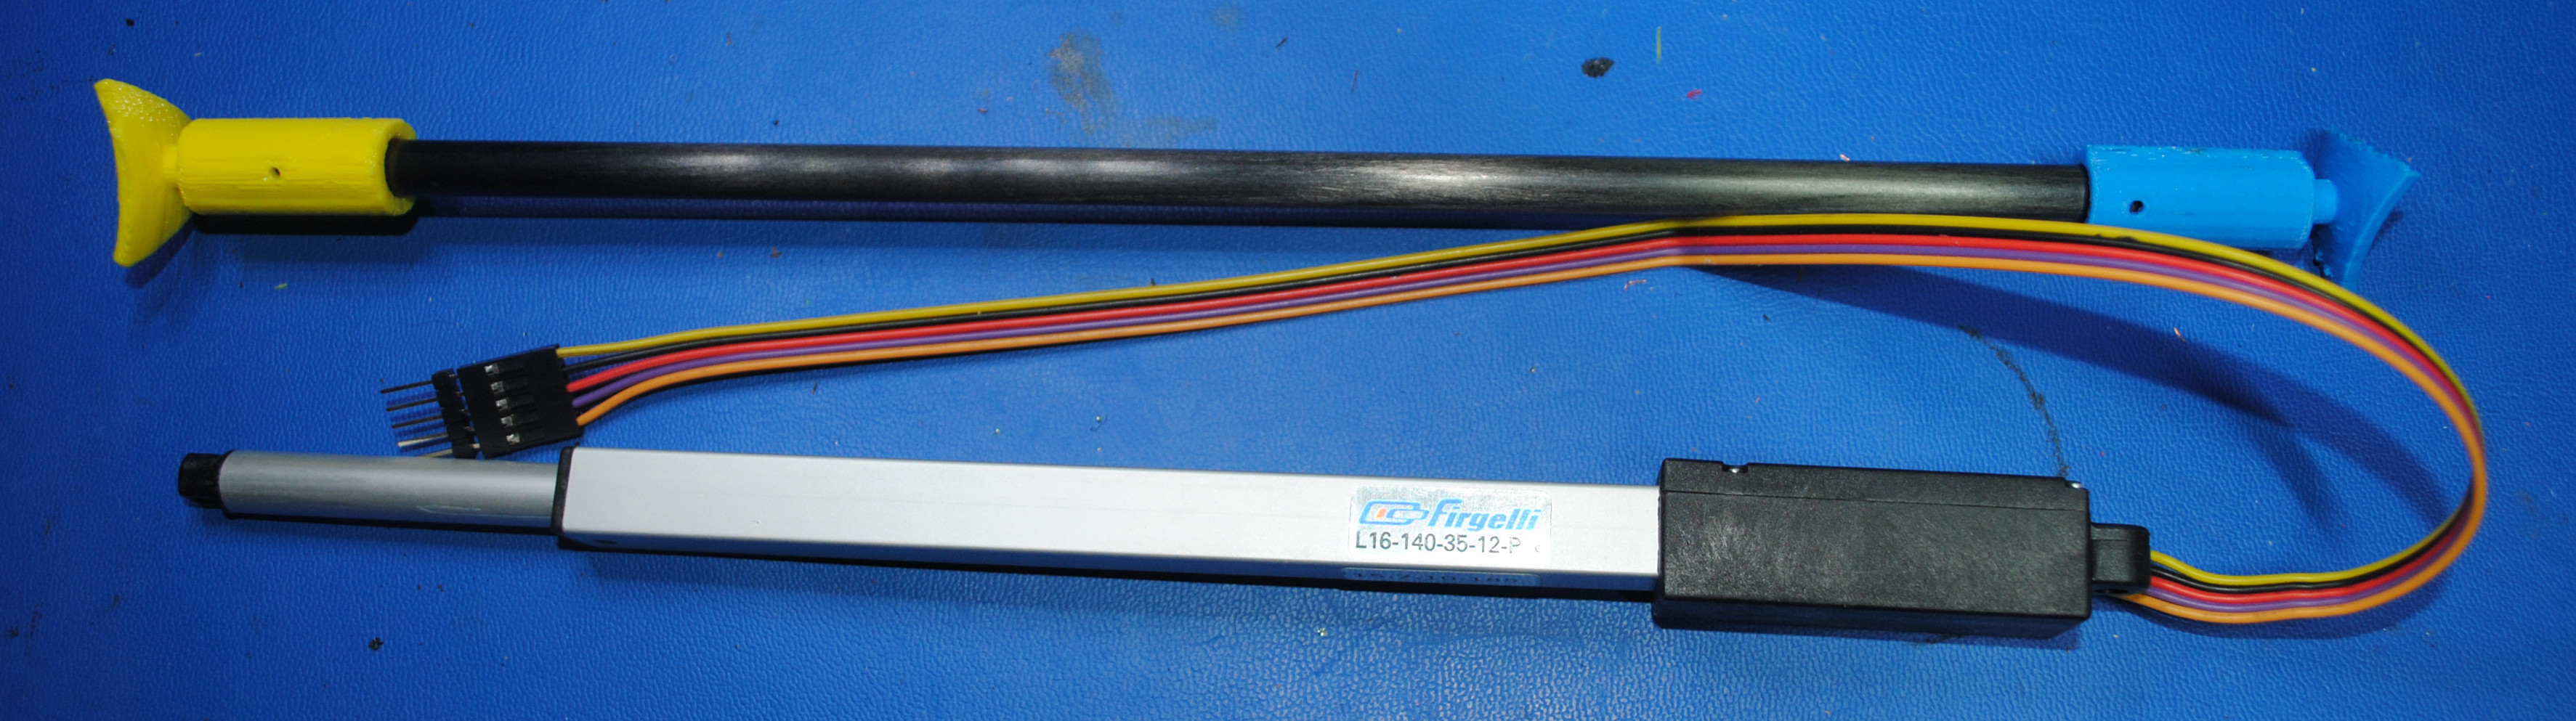
\includegraphics[width=1.0\textwidth]{figures/CarbonFiberAndActuator.jpg}
    \caption[Static Rod and Actuator]{Static Rod and Actuator}
      \label{rodAndActuator}
\end{figure}

We use the term Linear Actuator to refer to any device that is capable of changing its length. When
used in gluss it might be called a \emph{glussion}, a single particle of gluss. Our current gluss
uses a commercial linear actuator (the Firgelli/Actuonix\textsuperscript{TM} L-16-140-35-12-P,
\href{http://www.firgelli.com/L16_Linear_Actuators_p/l16-p.htm}{http://www.firgelli.com/L16\_Linear\_Actuators\_p/l16-p.htm}
)\footnote{At the time of this writing, Firgelli Technologies Inc. has changed its name to Actuonix Motion Devices.}
that costs about \$80 and exerts about 50 Newtons of force.
Turret joints that are 3D printed in plastic have been strong enough for this level of force.

However, in principle there is no reason we could not use the enormous hydraulic cylinders
used by backhoes, bullozers, and other earth moving equipment. These would of course require much
stronger joints. Probably not made out of plastic.

We could also attempt to make smaller actuators, to make a pocket-sized gluss. This is probably
a greater technical challenge, because it is relatively difficult to make small electric motors.

The current actuators use a rotary motor with a lead screw. This has the advantage of great
strength relative to their size, and of retaining position forcefully with relatively little backlash. It has the disadvantage
of being relatively slow. It would be interesting to build a gluss out of linear motors, for
example tubular linear synchronous motors. These would be much faster than the lead-screw type
actuators, resulting in a much faster gluss. 

\section{Control and Motion}
\subsection{Architecture of the 3TetGlussBot and 5TetGlussBot}

We have constructed what we believe to be the simplest possible Tetrahelix-based glussbot that is capable of locomotion
without relying on inertia.
It comprises:
\begin{itemize}  
\item 12 actuators,
\item 6 turret joints,
\item 2 12V battery packs, and
\item 2 controller units, each of which comprises:
\begin{itemize}  
\item 1 Arduino Mega microcontroller, and
\item 1 custom Arduino Mega shield hosting 6 1-amp motor channels and a BlueTooth module,
\end{itemize}  
\end{itemize}

Using these components, an NTetGlussBot can be constructed for any number of tetrahedra $N$

\begin{itemize}  
\item $(N + 1)\cdot 3$  actuators,
\item $N+3$ turret joints,
\item $\lceil \frac{N + 1}{2} \rceil$ 12V battery packs, and
\item $\lceil \frac{N + 1}{2} \rceil$ controller units,
\end{itemize}
for a cost of about \$400 per tetrahedra.


\begin{figure}[!ht]
  \centering
%%    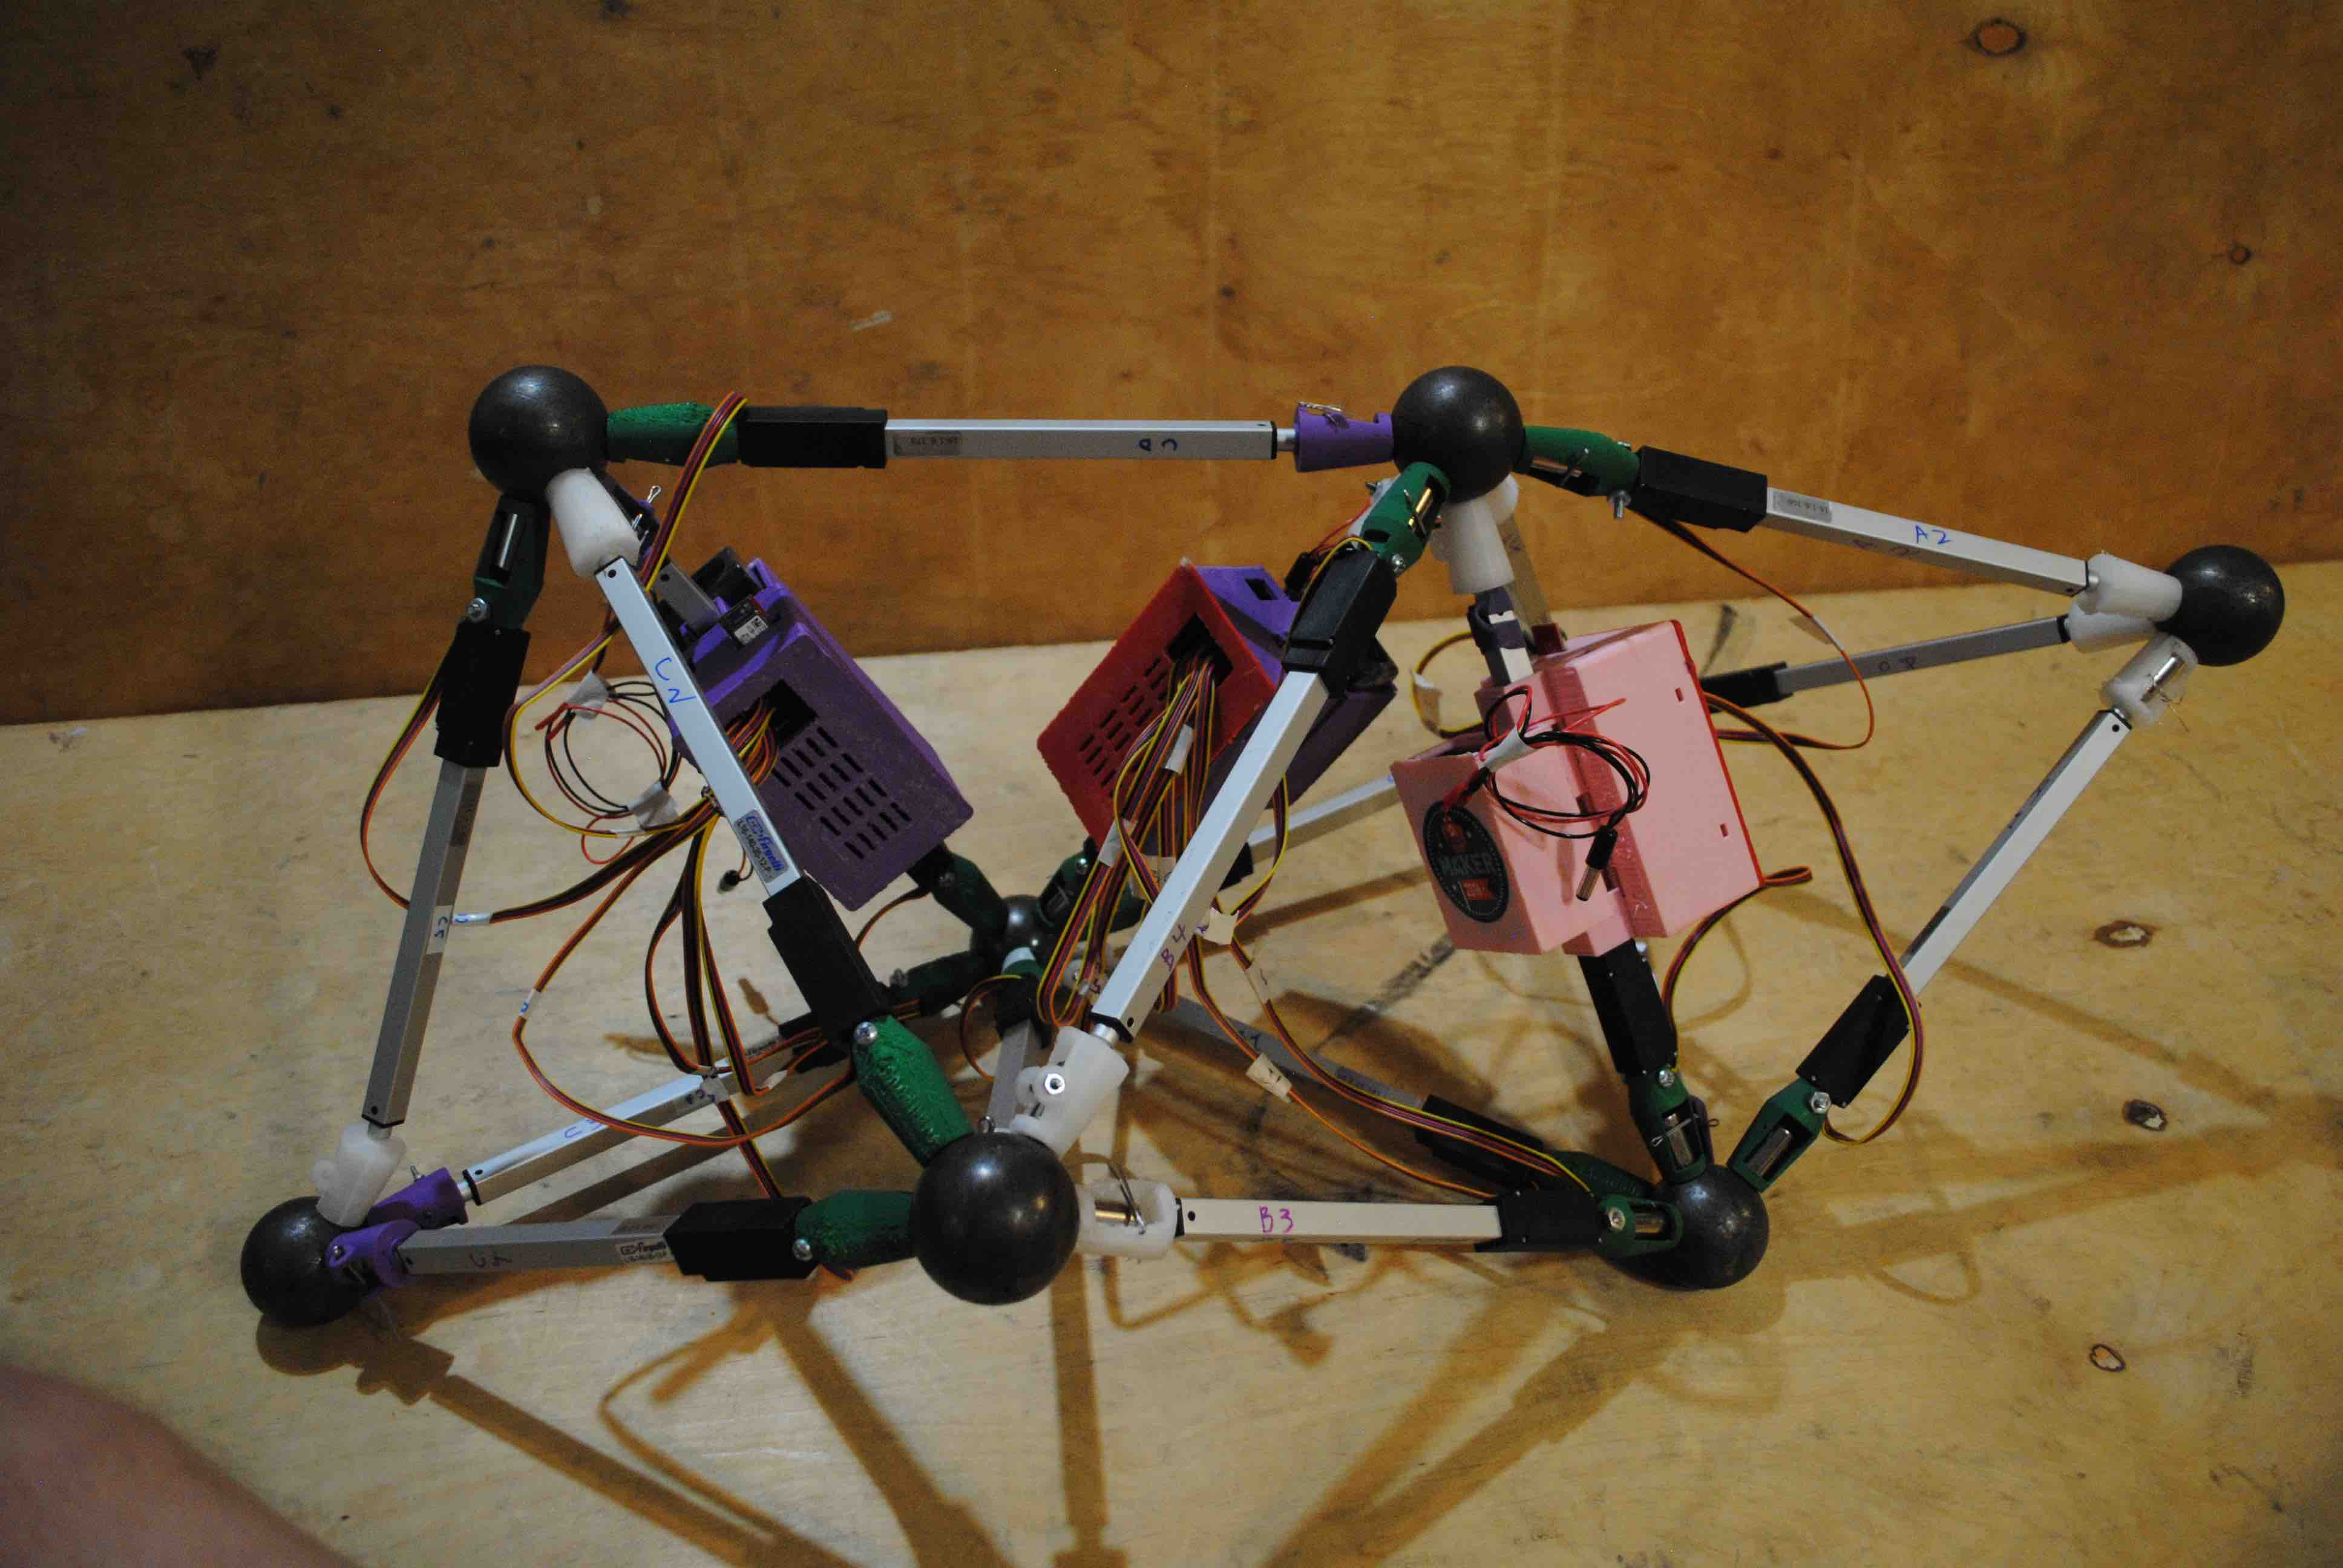
\includegraphics[width=0.8\textwidth]{figures/5TegGlussBotOverview.jpg}
    \caption[5TetGlussBot Components]{5TetGlussBot Components}
      \label{5TetGlussBot}
\end{figure}


Each controller module electrical system can support up to 6 actuators, so two are required for the 3TetGlussBot.
The BlueTooth modules open serial connections controlled by a computer.
The Arduino Mega is programmed to support commands addressed to each or all of the actuators, and
to provide feedback. The computer and the Arduino control programs communicate via S-Expressions
implemented with our own module. This is very analogous to sending JSON back and forth.

Commands to and feedback from the controller modules are managed by an Emacs E-Lisp program.
This program organizes motion into ``poses''. A series of poses make a ``dance''.
In order to dance, the program must synchronize the completion of poses, because there is no
guarantee how long it will take to achieve a pose. The time to reach a position in theory
depends on the voltage level provided by the battery and the force resisting the motion.
In practice, when lightly loaded by moving only itself, the time is relatively predictable. It takes
about 3 seconds for the 3TetGlussBot to go from its most compact state to its largest, most expanded state.

The current software has been written in anticipation of a much larger number of controllers and much more gluss.
Nonetheless as mentioned in Section \ref{futuresteps} the current software is specific to either the 3-tetrahedron geometry or the
5-tet geometry.


\subsection{Open Source Realizations}

We have provided everything necessary to construct gluss in the form of FLOSS. Providing an ``Instructable''-style
how-to guide is beyond the scope of this article, but a semi-skilled electronics hobbyist can use the
following resources to construct their own GlussBot.

\begin{description}
  
\item [Turret Joint]
  The Turret Joint is implemented via OpenSCAD files. The file itself is here:\\
  \href{https://github.com/PubInv/turret-joint/blob/master/Models/TurretJoint.scad}
       {https://github.com/PubInv/turret-joint/blob/master/Models/TurretJoint.scad}.
       The model may be observed without even installing OpenSCAD, and even 3D printed,
       from the same file using the customizer feature of Thingiverse.\\
       \href{http://www.thingiverse.com/thing:1043716}{http://www.thingiverse.com/thing:1043716}
  
\item [Robot Controller Shield]
  An Arduino Mega Shield may be ordered directly from OshPark and then hand-soldered with through-hole components,
  where it is titled the \emph{3x2 Motor Controller MegaShield, v0.2}.
  The \href{https://oshpark.com/shared_projects/fijpozoB}{https://oshpark.com/shared\_projects/fijpozoB} shield
  may be useful to anyone who wants to control up to six DC motors (up to 1 amp each) at the same time, via Bluetooth.
  Alternatively, you may use the Creative Commons-licensed Eagle Soft CAD files, which can be found here:
  \href{https://github.com/PubInv/gluss/tree/master/GlussPCBv0.1}
  {https://github.com/PubInv/gluss/tree/master/GlussPCBv0.1}
   \begin{figure}[!ht]
     \centering
%%     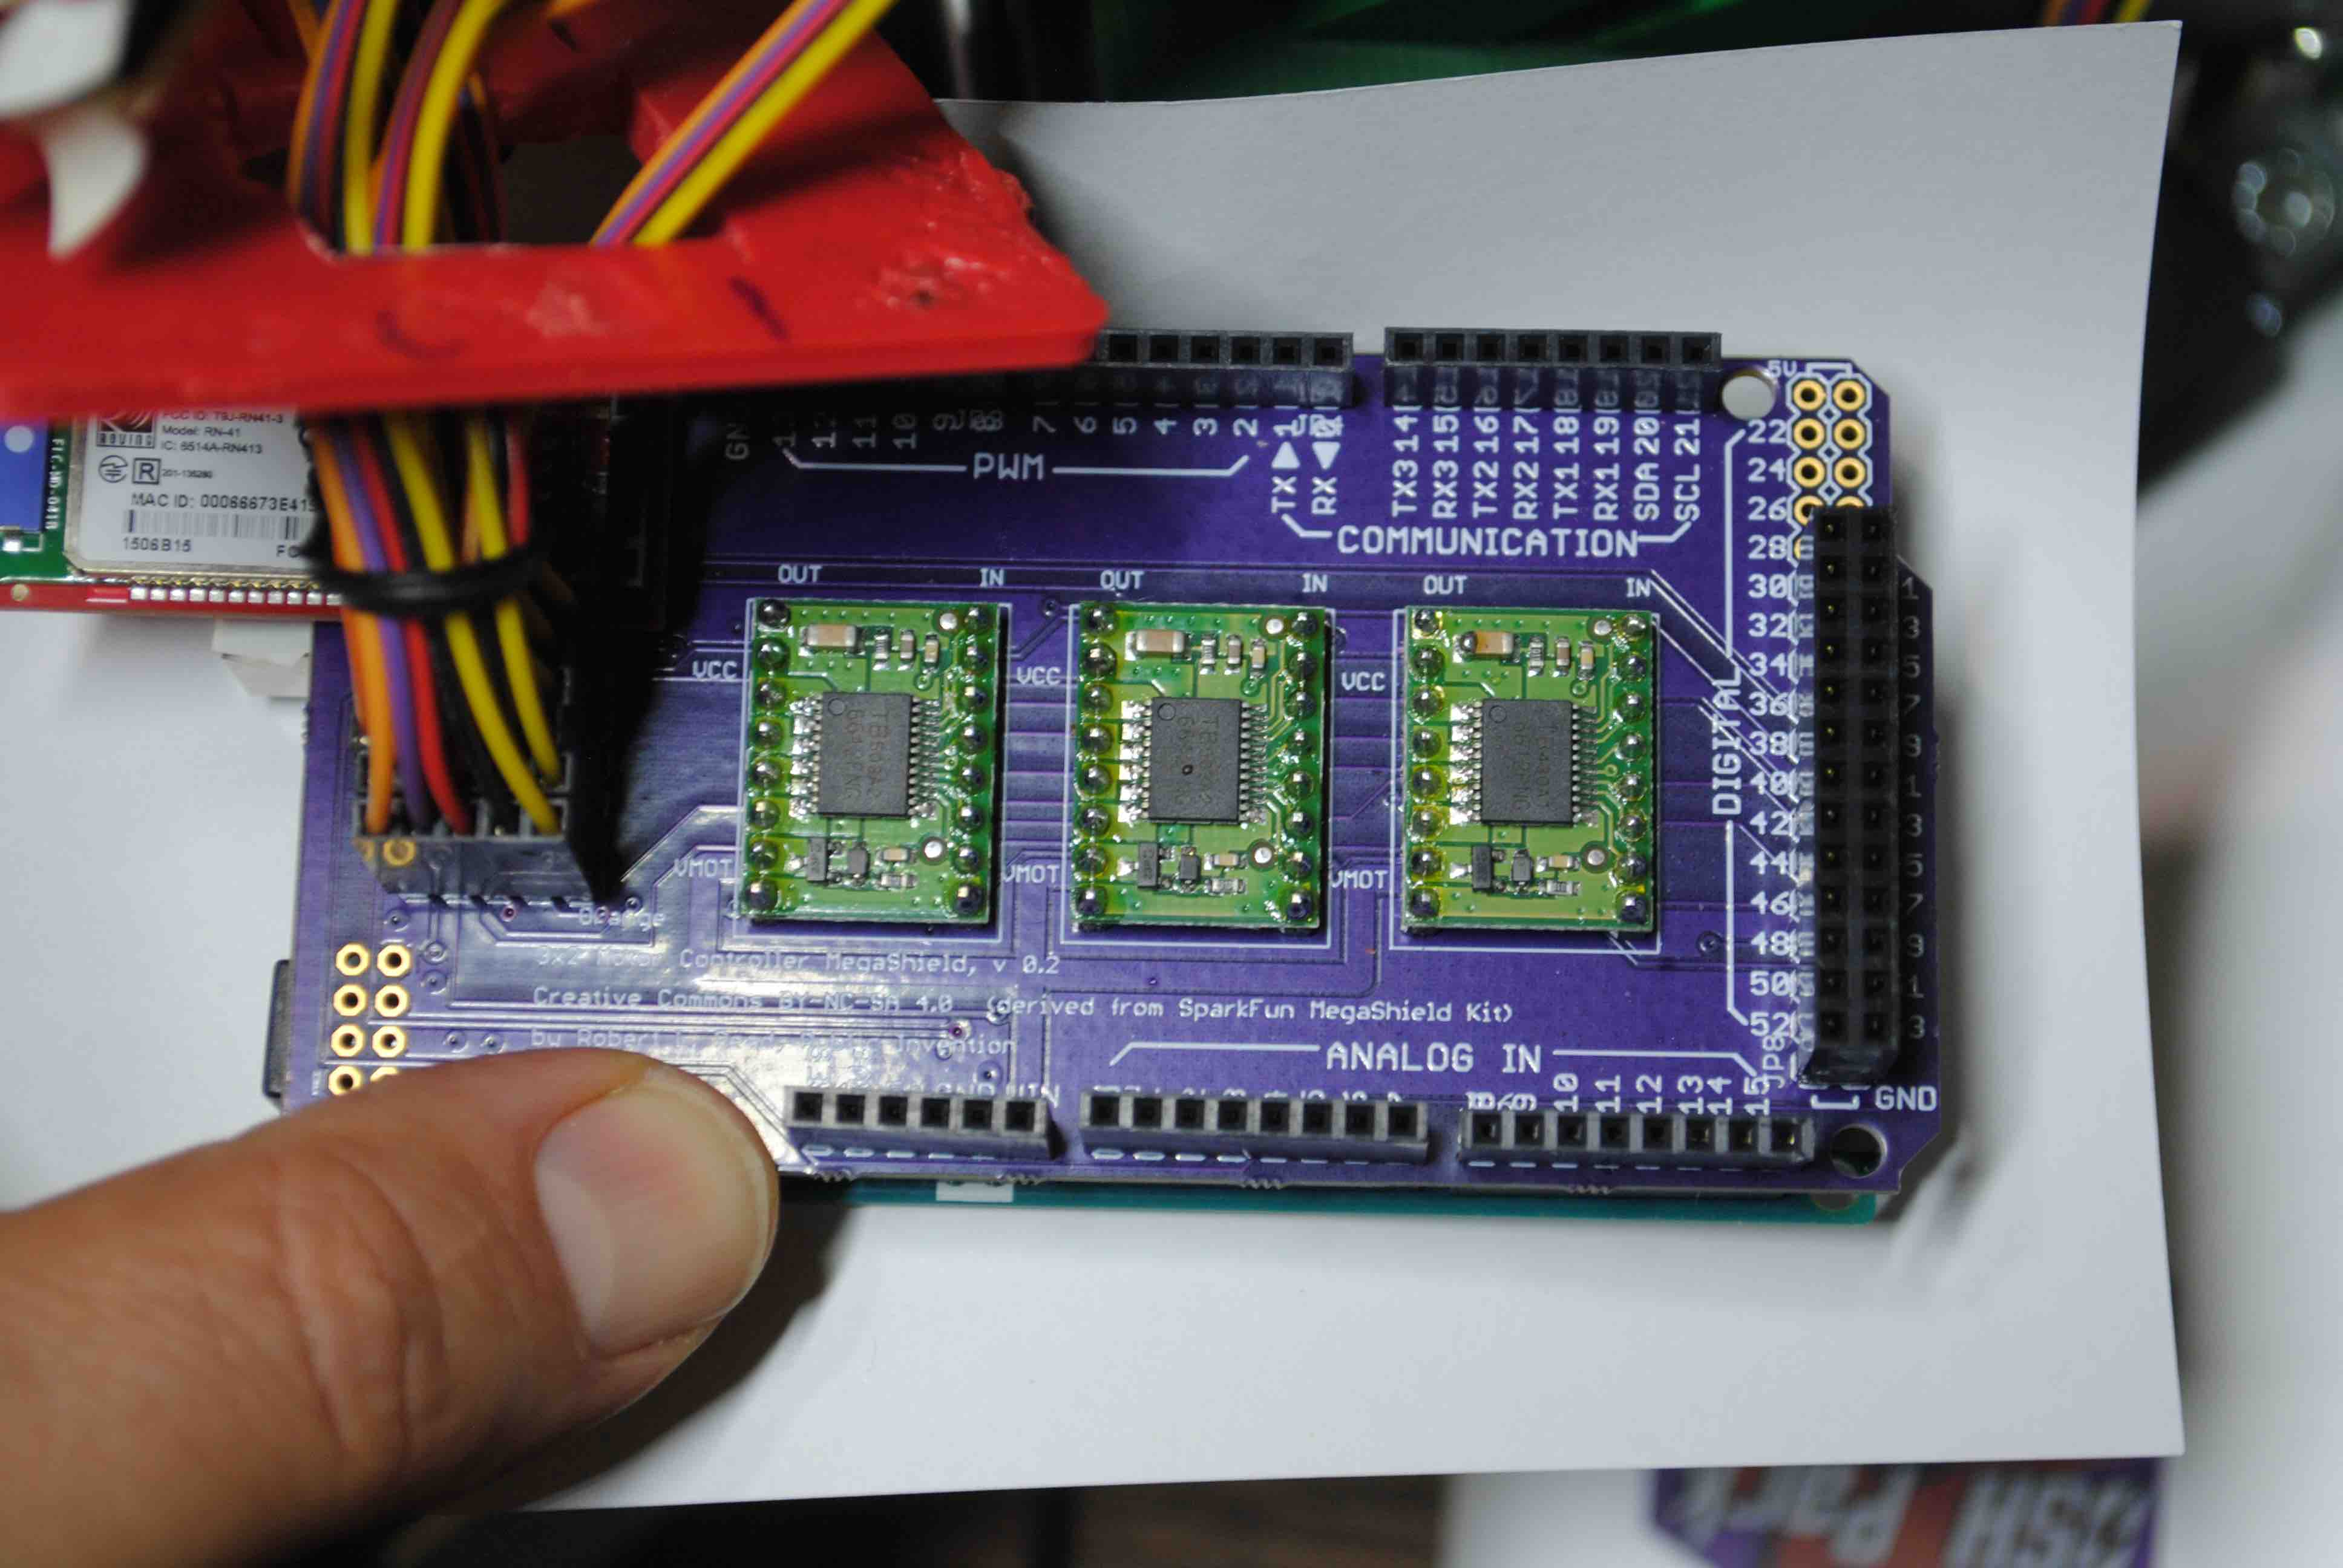
\includegraphics[width=0.5\textwidth]{figures/MotorControllerInPlace.JPG}
     \caption{Arduino Mega Shield board}
   \end{figure}

\item [Mountable Enclosures]
  Files to 3D Print the mountable enclosures for the battery pack and the Arduino Mega with the Robot Controller Shield are:\\
  \href{https://github.com/PubInv/gluss/tree/master/MegaAndShieldEnclosure}{https://github.com/PubInv/gluss/tree/master/MegaAndShieldEnclosure}

\item [Control Software]
An Emacs LISP program which controls the 3TetGlussBot via a command-line interface:
\href{https://github.com/PubInv/gluss/blob/master/emacs-ctl.el}{https://github.com/PubInv/gluss/blob/master/emacs-ctl.el}

An Arduino Sketch which implements a device driver for the GlussBot Controller Shield is required as well:

\href{https://github.com/PubInv/gluss/blob/master/GlussPCBv0.1/GlussPCBv0.1.ino}
     {https://github.com/PubInv/gluss/blob/master/GlussPCBv0.1/GlussPCBv0.1.ino}.
     This sketch needs the Arduino module S-Expr.
     
\item [S-Expr]
  The \href{https://github.com/PubInv/S-Expr}{https://github.com/PubInv/S-Expr} Arduino S-Expr project and its
  test project
  \href{https://github.com/PubInv/Arduino-S-Expr-Test}{https://github.com/PubInv/Arduino-S-Expr-Test} 
  may be useful to anyone who wants to control an Arduino from Lisp or prefer S-Expressions to the closely related JSON format.

  
\end{description}

\subsection{Speed Performance}

The 3TetGlussBot is capable of ``walking'' and turning. Some might prefer the term ``crawl'' to ``walk'' in
this case. It can move forward awkwardly at a rate
of about five inches per minute. It can turn 30 degrees in about 60 seconds.
We believe the 3TetGlussBot is the simplest amount of gluss that would be capable of locomotion.

The present mode of walking avoids dragging the pseudopods by leaning to one side or front or back and
then lifting the pseudopod, moving it forward (without ground contact), and placing it down again.
Such a gait may be able to handle rugged terrain better than a gait that drags. Furthermore, the
3TetGlussBot gait assumes and has no anisotropy of friction against the ground, as is typical
of snakebots.
It is also non-inertial, in that it simply assumes that the actuators are powerful enough to
move to any extent commanded of them. No attempt to model force has thus been made in the control of this gait.
Since the gait was constructed by hand, it does not represent a modelling of the idea of leaning and or
unweighting a given joint.

The 5TetGlussBot is significantly faster, moving about 7.5 inches per minute in the ``broadwalk'' mode
and about approximately 28 centimeters per minutes (11 inches per minute) in a walk in the ``thin'' direction using a ``slide'' in its gait.

The current programmed gaits are not optimal.
We are developing a browser-based simulation using the Cannon.js physics engine that should allow for development
of more efficient gaits without having to actually have a robot.

\section{Related Research}

Between 14 and 21 years ago, Arthur C. Sanderson and his colleagues published a series of
papers\cite{sanderson1996modular,lee2002dynamic,lee1999dynamics} on modular robots.
The ``TETROBOT'' was a variable-geometry truss, in which motion was accomplished but the change
in length of linear actuators, connected in a modular geometry based on the tetrahedron and octahedron.
A quadrupedal robot was constructed completely out of the tetrahedral/octahedral geometry.
The TETROBOT robots successfully walked and even rolled. The TETROBOT hardware was significantly
heavier and more powerful that then hardware used here. The glussbots have so far demonstrated no greater functionality,
although we have demonstrated that very simple robots consiting of only 3 tetrahedra can locomote.

The present article has drastically lowered the cost thus making the glussbot/TETROBOT concept
accessible to hobbyists and researchers on a tight budget.

The TETROBOT used a joint called the \emph{concentric multilink spherical} (CMS) joint. Although
possibly superior in not allowing an extra degree or rotational freedom, it would be a challenge to use the CMS
joint with the Actuonix\textsuperscript{TM} actuators because the pushrod must fully retract, or the length of the pushrod would be
have to be extended with an attachment. Prof. Sanderson's students used actuators that
extended from the middle, avoiding this problem. If the Gluss Project ever develops its own actuators, it should
explore using this joint.

If you read the introduction of the brilliant book by Shigoe Hirose\cite{hirose1993biologically} substituting
``even simpler soft squiggly thing that might not be as cylindrical as a snake'' for the word ``snake'', you will have
an excellent motivation for the gluss concept.  More generally, much of the work developed for snakebot
locomotion\cite{liljebäck2012snake} is directly reusable, in the sense that a long enough tetrahelix can
model a snake, and further inspires the idea of using simpler models mapped into a gluss model to perform
complex movements.

Buckminster Fuller also promoted \emph{tensegrity}, and some research on Tensegrity Robots has been done, the
work of Paul, Valero-Cuevas, and Lipson\cite{paul2006} being a good starting point.
This work has developed into a serious effort by NASA to explore tensegrity robots for extraterrestrial
exploration.

Tensegrities are closely related to the gluss concept, more researched, and potentially more performant.
In fact a gluss could be considered a special case of a tensegrity, using vanishingly short cables
and, in the terminology of \cite{paul2006}, \emph{strut-collocated actuation}.
In spirit, however, the difference is that a tensegrity is lighter, more flexible, and more dynamic.
It has been reasonable to produce a static gait for the 3TetGlussBot and 5TetGlussBot because its behavior is not
very dynamic: it is so slow and strong that velocity is irrelevant at the current scale.

It is possible that gluss is easier to work with for an actual human being on the ground.
Although of course both systems will use computer control systems, one can imagine a large robot
crawling into place imperfectly, and some workperson making a manual adjustment: ``Actuator \#37, get shorter!''
This is probably harder for a tensegrity, which seems to me less intellectually natural.  However, many
of the future steps outlined in Section \ref{futuresteps} apply to both gluss and tensegrity robots.

This paper presents the gluss as a ``machine'', rather than a ``mechanism''. That is, it motivates gluss
by asserting it can exert and resist force, yet currently treats gluss positioning as a purely kinematic,
rather than dynamic problem. The actuators currently in use are geared such that they are so slow
and powerful that the behavior is not really dynamic. Classic control theory has not yet been needed.
As the gluss is made larger and longer and dynamics are added,
a finite element approach\cite{géradin2001flexible} seems appropriate,
given its ability to represent complex structural connections and static analysis.



\section{Future Steps}
\label{futuresteps}

Actions are available at the research level and at the hobbyist level, and we refuse to draw
a crisp distinction between the two, but we have organized these from most difficult to least
difficult.

\begin{description}
\item [Remove Scale:] (Pure math, physics, computer science) At present the 3- and 5-TetGlussBot is programmed
  as a specific geometry. Any program
  written for it would have zero value for a robot of the same general shape but built with considerably
  more actuators. Ideally, we would be able to program gluss completely independent of the scale
  of implementation. We would treat it as a true metamorphic material, rather than as a net of
  actuators arranged in a particular configuration. This can be considered a problem of pure
  mathematics, touching on wavelet theory, for example. It blends into computer science and
  finally robotics.
\item [Math of Ideal Systems:] (Geometry) What configurations are possible of ideal and real-world gluss?
  For example, what is the maximum radius of curvature of an octet truss employing joints
  and actuators of specific properties? This is primarily in the realm of geometry, and perhaps
  computational geometry.
\item [Throw a Ball:] (Mechatronics) Develop the dynamic control needed to throw a ball, thereby moving from
  kinematics to dynamics.
\item [Cheap Actuator:] (Physics, Electrical Engineering) The gluss concept heightens the need for very inexpensive linear
  actuators. The current actuators at \$80 make constructing a 100-actuator glussbot expensive.
  It should be possible to build a linear actuator for 1/10th of this cost, although it may require
  giving up some advantages. If we imagine a design spectrum of actuators, creating a new and
  less expensive point in the spectrum of actuators designs would greatly
  expand the possibilities of gluss.
\item [Applications:] (Philosophy, Design, Entrepreneurship) A killer application would help motivate the gluss concept. This does not
  require engineering, but requires careful thought.
\item [Static Force Performance:] (Structural Analysis)
It would be be nice to answer the questions such as:
\begin{itemize}  
\item If a 5-tetrahedron tetrahelix were bolted to a frame and extended horizontally, how much
  weight can it support at the free end?
\item If a gluss bot crawled under a car and sought to jack up the car enough for a tire
  to be changed, how forceful would each actuator have to be?
\item If a large glussbot crawled across a chasm, could a truck or a human being safely move
  across it without danger of collapse?
\end{itemize}
We have not attempted to analyze gluss in terms of force performance. We believe this would
be analogous to analysis of static space frames using the dynamic configuration at a point.
Finite element analysis is a standard approach to this.
\item [Quick Joint:] (Mechanical Engineering) If all of the turret joints in a 3TetGlussBot are disassembled so that
  the linear actuators can be stacked together for efficient transport, it takes more than an hour
  to bolt them back together. It would be very convenient to have a joint that could be
  disassembled and assembled more quickly. We have found that it is possible to build a magnetic
  joint similar (but larger) than those used in the Geomag\textsuperscript{TM} toy. However, it does not scale up in size
  and is weak against side forces. We would like to investigate the turret joint using bolt-free ``bayonet mounts'' which
  can be easily snapped into place.
\item [Construction System:] (Mechanical Engineering) If we imagine the members connecting the joints are not actuators but
  simply rods that can be cut to any length, we have a construction system for making spaceframes.
  Explore the possibilities of such a construction system to make organic and interesting shapes
  freed of rectilinear limits.
\item [Build Simulator:] (Computer Science) A 3TetGlussBot can be constructed for about \$1300. Nonetheless this
  is beyond the means of many hobbyist. A simulator would allow one to research 
  motion without monetary cost. The open-source, browser deliverable physics engine ``Cannon.js''
  provides all the basic machinery needed to build such a simulator.
\end{description}


\section{Contact and Getting Involved}

The Gluss Project \href{http://pubinv.github.io/gluss/}{http://pubinv.github.io/gluss/}
is a free-libre, open-source research, hardware, and software project that welcomes volunteers.
It is our goal to organize projects for the benefit of all humanity without seeking profit or intellectual property.
To assist, contact \href{mailto:read.robert@gmail.com}{$<$read.robert@gmail.com$>$}.

\bibliographystyle{IEEEtran}
\bibliography{IEEEabrv,gluss}



%% \newpage



%% \appendix

%% \section{Turret Joint Geometric Limitations}

%% \label{phiproof}

%% \subsection{Geometric Preparation}



%% Defining all angles against a center line between two rotor holes in a plane,
%% let:

%% $ A \equiv $ Min Actuator Length. Without loss of generality, assume this is $ 1.0 $.

%% $ Z \equiv $ Max Actuator Length

%% $ Q \equiv \frac{Z}{A} $, The ratio of the actuator lengths, noting that $Q \geq 1$. Since $A = 1$, $Q \equiv Z$.

%% $ G \equiv $ Greatest Angle Reachable by Center of Rotor

%% $ L \equiv $ Least Angle Reachable by Center of Rotor

%% $ P \equiv $ Angle from the Post to the edge of the Rotor

%% $ \theta \equiv $ Angle of Inmost Edge of the Rotor Hole

%% $ \psi \equiv $ Angle of Outmost Edge of the Rotor Hole



%% \begin{figure}[!ht]
%%   \centering
%%     \includegraphics[width=0.5\textwidth]{figuresConstraintDrawing.png}
%%     \caption[Constraints]{Turret Joint Geometry Constraints}
%%       \label{constraint-drawing}
%% \end{figure}

%% \bigskip

%% What $\theta, \psi$ maximizes $Q$ and what is $Q$?

%% \bigskip

%% We will define the angle of the hole to be:

%% \[\tag{Delta Definition} \Delta \equiv \psi - \theta \]

%% From the diagram:


%% We then place engineering constraints upon these variables to represent physical conditions
%% which define the limits of the joint.
%% We name these constraints \textit{meet}, \textit{bump}, \textit{capture}.

%% The \textit{meet} condition means that post is actually within the hole.

%% The \textit{bump} condition means that the rotors don't bump into each other
%% in their extreme position.

%% The \textit{capture} condition means that the the rotor can't fall out of the hole.

%% In both cases, we have have the capture constraint:

%% \[ \tag{capture} \Delta \geq G - L \]

%% To realize the most acute position, we have constraints:

%% \[ \tag{acute meet} \theta \leq L \]

%% \[ \tag{acute bump} \frac{\Delta}{2} \leq \theta  \]

%% To realize the least acute position, we have constraints:

%% \[ \tag{obtuse meet}  \psi \leq G \]

%% It is perhaps obvious that the rotors cannot bump in the most obtuse position, but we observe that:

%% \[ \tag{obtuse bump} 360\degree - 2\cdot \psi \geq \frac{G - L}{2} \]

%% is invariably true because $2\cdot\psi < 180\degree$ because psi is a half angle of a triangle, and likewise $\frac{G - L}{2} < 180\degree$.

%% \subsection{Maximum usable Q = $\varphi$}

%% In the previous subsection we set up geometric conditions generally so that we could consider them from
%% both a Classical Trigonometry and from Rational Trigonometry.  Although we used the world ``angle'', we did not
%% rely additive properties of angles except in the definition of Delta and the ``obtuse bump'' condition.  This will allow us
%% to perform an analysis in Rational Trigonometry in the next section.

%% When we attempt to set $G$ and $L$ to be as wide apart as possible by asserting $G \equiv \psi$ and $L \equiv \theta$, we must
%% ensure that all of thse constaints are true. The two meet conditions become true by equality. Likewise the capture condition
%% is trivially true by substitution. The obtuse bump condition can
%% never be false.  However, the acute bump conditions remains:

%% \[ \tag{acute bump} \frac{\Delta}{2} \leq \theta  \quad \equiv \quad \frac{G - L}{2} \leq L  \quad \equiv \quad G \leq 3 \cdot L \]

%% \[
%% G \equiv \arcsin{\frac{Q}{2}}
%% \]
%% \[
%% L \equiv \arcsin{\frac{1}{Q \cdot 2}}
%% \]

%% Returning to our definitions of G and L,

%% \[ \arcsin{\frac{Q}{2}} \leq 3 \cdot \arcsin{\frac{1}{Q \cdot 2}} \]

%% So our question becomes what is the maximum $Q$ that satisfies this inequality. Noting from the graph of the $\arcsin$ function in
%% the relevant ranges where $Q \geq 1$ that $G$ is a monotonically increasing function and $L$ is a
%% monotonically decreasing function of $Q$ (since $Q$ is in the denominator), the maximum $Q$ will be the solution to:

%% \[\tag{original}  \arcsin{\frac{Q}{2}} = 3 \cdot \arcsin{\frac{1}{Q \cdot 2}} \]

%% Upon investigating this with a spreadsheet we noted that Q suspiciously approached the famous number 1.618..., the golden ratio, $\varphi$.
%% We investigated further with the help of Wolfram Alpha Pro
%% (\href{https://www.wolframalpha.com}{https://www.wolframalpha.com}).
%% Wolfram Alpha gave us a closed-form solution to \emph{original} of $\frac{1 + \sqrt{5}}{2}$
%% that we recognized as $\varphi$, but oddly would
%% not show us the set of transformations. After verifying that $Q = \varphi$ was
%% a solution in that way, we used the special property of
%% $\varphi$ that $ \varphi = \frac{1}{\varphi} + 1 $, to rewrite our constaint as:

%% \[\tag{assuming $Q=\varphi$} \arcsin{\frac{Q}{2}} = 3 \cdot \arcsin{\frac{Q - 1}{2}} \]

%% which led Wolfram Alpha Pro to indeed provide a long and complex chain of trigonometric transformations to show that
%% $Q \equiv \frac{1 + \sqrt{5}}{2} \equiv \varphi$ is actually an algebraic solution to
%% this equation.

%% Thus the surprising result is obtained that, for a turret joint where the problem of the rotors physically bumping is not
%% solved by some other means, the highest $Q$ that we can take advantage of is $\varphi$, and that it would be
%% perfectly correct in Figure \ref{constraint-drawing} to label the slenderest triangle as a Golden Triangle and the obtuse
%% triangle as a Golden Gnomon. Furthermore, $\theta = 18\degree$, and $\psi = 54\degree$, and $\Delta = 36\degree$.

%% This is a valuable ideal to strive for, but a physically realizable joint may not support such a high $Q$,
%% because any naive physically realizable
%% turret joint is likely to have a rotor diameter with a lip significantly larger than the hole, and the post will have an actual
%% thickness that must be considered in computing $G$ and $L$. Nonetheless this analysis is a starting point for analyzing more
%% realistic joints, even if such joints will have to be dealt with numerically rather than having an elegant analytic solution.

%% \label{rationalphiproof}

%% \subsection{Rational Trigonometry}

%% A magician may pull a rabbit out of a hat, but a mathematician should avoid it.
%% The Classical Trigonometry result in the last section feels like pulling a rabbit out of a hat because it relies
%% on results beyond our ability of human calculation.  Norman J. Wildberger has a presented a simpler re-formulation
%% of trigonometry called Rational Trigonometry\cite{wildberger2005} that proposes to avoid such rabbits.

%% This section assumes the reader is familiar with Rational Trigonometry.

%% In our diagram and our previous formulation, we can almost treat the angles of that diagrams as spreads. However,
%% since spreads are non-linear, we cannot use \textit{Delta Definition},  or \textit{acute bump} in their
%% formulation from that section.


%% Now if we consider $theta$, $G$ and $L$ as spreads, we have the definition of the spread as the quadrance of the
%% opposite leg over the quadrance of the hypotenuse:


%% \[ \tag{rational-theta} \theta \quad \equiv \quad \frac{(1/2)^2}{Q^2} \quad \equiv \quad \frac{1}{4 \cdot Q^2}  \]

%% \[ \tag{rational-psi} \psi \quad \equiv \quad (\frac{Q}{2})^2 \quad \equiv \quad \frac{Q^2}{4}  \]


%% Rather we assert to avoid the problem of the rotors bumping in the case of the most acute triangle we assert:

%% \[ \tag{rational acute bump} P \leq \theta  \]

%% Our goal is to find the maximum Q satisfying all constraints.  It is clear that $\theta$ goes down as $Q$ goes
%% up, and that $\psi$ goes up as $Q$ goes up.  $P$ goes up as $Q$ goes up (this remains to be rigorously shown).

%% Therefore $Q$ is maximized when $P = \theta$.

%% We can thus use Theorem 56 (Three equal spreads) \cite{wildberger2005} on $\theta$:

%% \[  \psi \equiv \theta (3 - 4 \cdot \theta)^2  \]

%% together with \textit{rational-psi} via substitution to obtain a series of purely algebraic manipulations:

%% \[  \frac{Q^2}{4} = \theta (3 - 4 \cdot \theta)^2  \]

%% then by substituting \textit{rational-theta}:

%% \[  \frac{Q^2}{4} = \frac{1}{4 \cdot Q^2} (3 - 4 \cdot \frac{1}{4 \cdot Q^2})^2  \]

%% performing elementary algebraic simplification we obtain:

%% \[  Q^4 = (3 - \frac{1}{Q^2})^2   \]

%% Perform the substitution $x = Q^2$:

%% \[  x^2 = (3 - \frac{1}{x})^2   \]

%% Take the square root of both sides and converting to common fraction:

%% \[  x = \pm \frac{(3\cdot x - 1)}{x}   \]

%% Cross multiplying and simplifying:
%% \[  x^2 - 3\cdot x =  - 1   \]

%% Completing the square by adding $\frac{9}{4}$ to both sides:
%% \[  x^2 - 3\cdot x + \frac{9}{4} =  \frac{5}{4}   \]

%% Writing left hand side as a square:

%% \[  (x- \frac{3}{2})^2 =  \frac{5}{4}   \]

%% Take the square root of both sides:

%% \[  \pm (x- \frac{3}{2}) =  \pm \frac{\sqrt{5}}{2}   \]

%% Adding $\frac{3}{2}$ to both sides:

%% \[  x =   1 + \frac{1}{2} + \frac{\sqrt{5}}{2}   \]

%% Being previously alerted to the existing of $\varphi$ in our solution, we recognize
%% this as $1 + \varphi = \varphi^2$. 

%% \[  Q = \sqrt{x}  =   \sqrt{1 + \varphi}  \]

%% Substituting back into $x = Q ^ 2$,

%% \[  Q =   \varphi  \]

%% Note that we have taken square roots twice in this operation, and therefore must
%% check that the negative solutions are not also valid solutions. Wolfram Alpha Pro
%% combined with the fact that only $Q > 1.0$ allows us to conclude this is the
%% only valid solution.

%% We have thus obtained the same algebraic result as the trigonometrical more understandably
%% and with less recourse to computer aids.

\end{document}

